\section{Vertical \& Lateral Connectivity {
\includegraphics[height=15pt]{connectivity-yz-small}}}

\subsection{Vertical Disconnectivity: Riverbed Clogging}

\begin{frame}{\secname\vspace{0.1cm}\\\textcolor{anthrazit!80!white}{\subsecname}}
	\begin{tikzpicture}
		\clip (0,0) rectangle (\paperwidth,\paperheight);
		\onslide<1->{
		\begin{scope}
				\node[anchor=south west, xshift=0.0\paperwidth, yshift=0.62\paperheight] {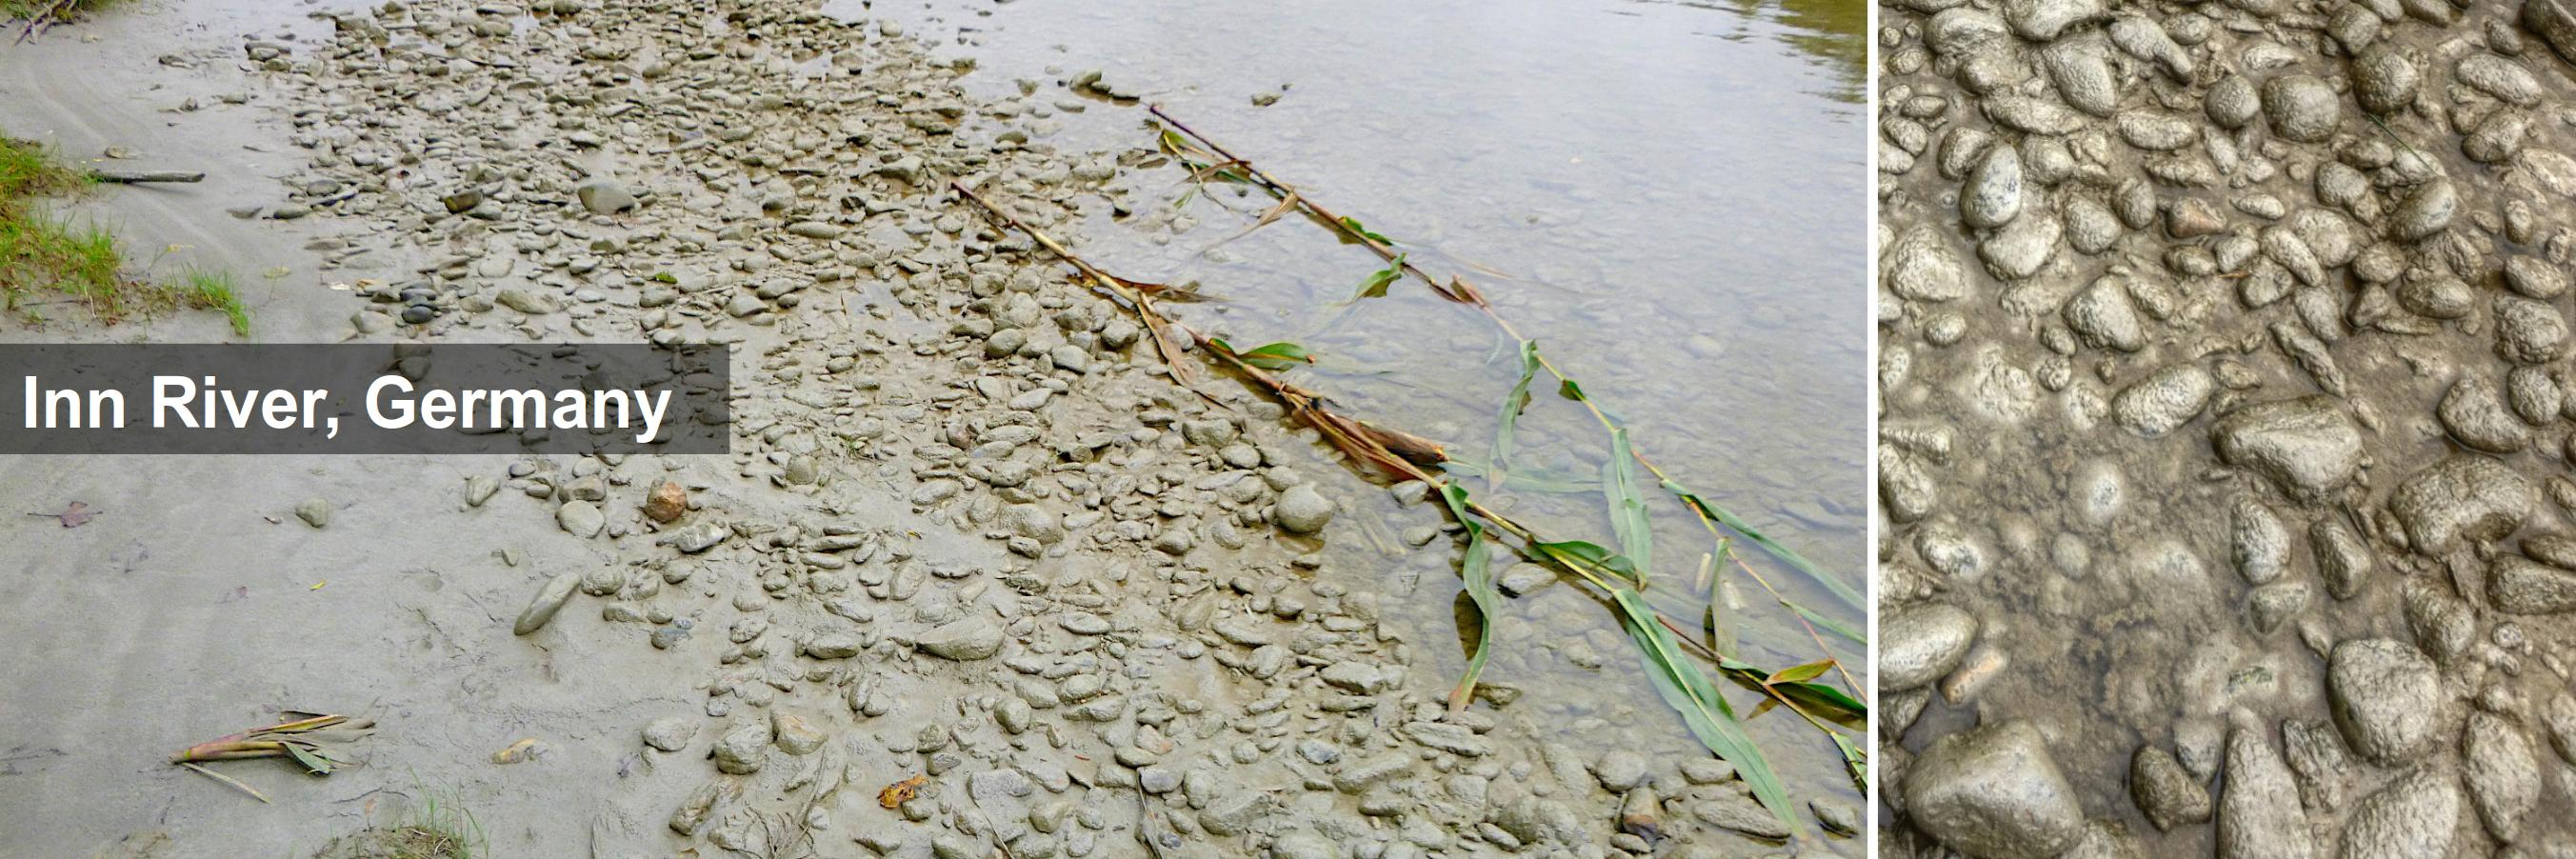
\includegraphics[width=0.91\paperwidth]{inn-clogging}};
		\end{scope}}
		\onslide<2-2>{
		\begin{scope}
			\node[anchor=south west, xshift=0.0\paperwidth, yshift=0.3\paperheight] {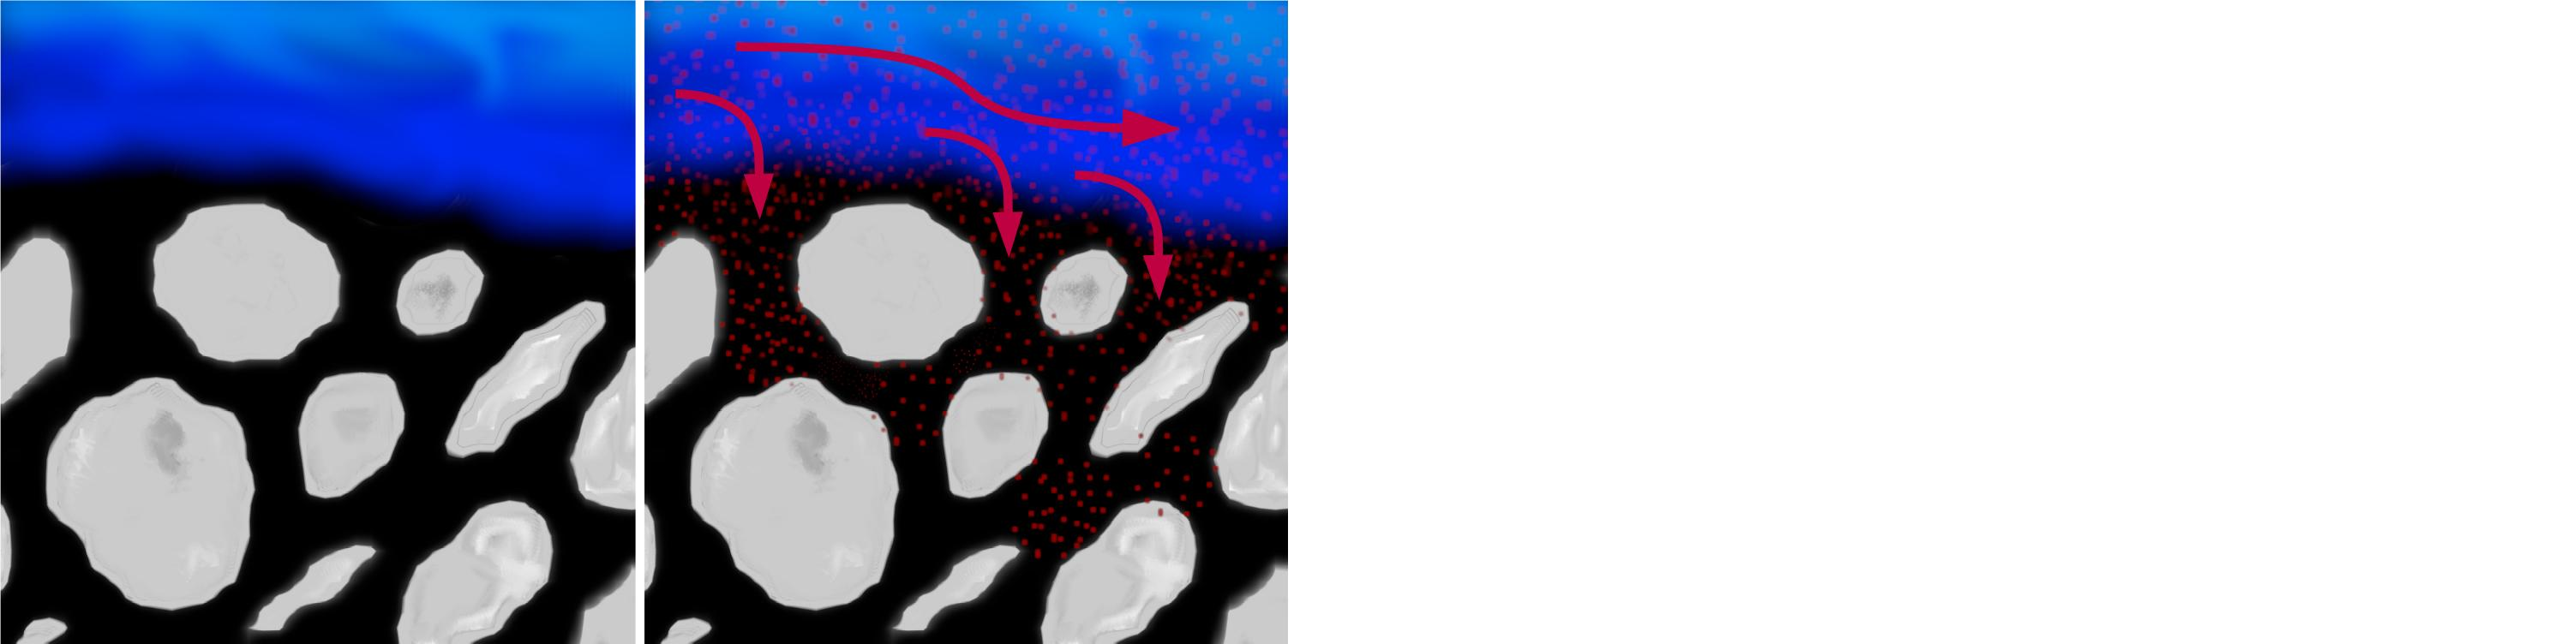
\includegraphics[width=0.91\paperwidth]{new-clogging-assembley-0}};
		\end{scope}}
		\onslide<3->{
			\begin{scope}
				\node[anchor=south west, xshift=0.0\paperwidth, yshift=0.3\paperheight] {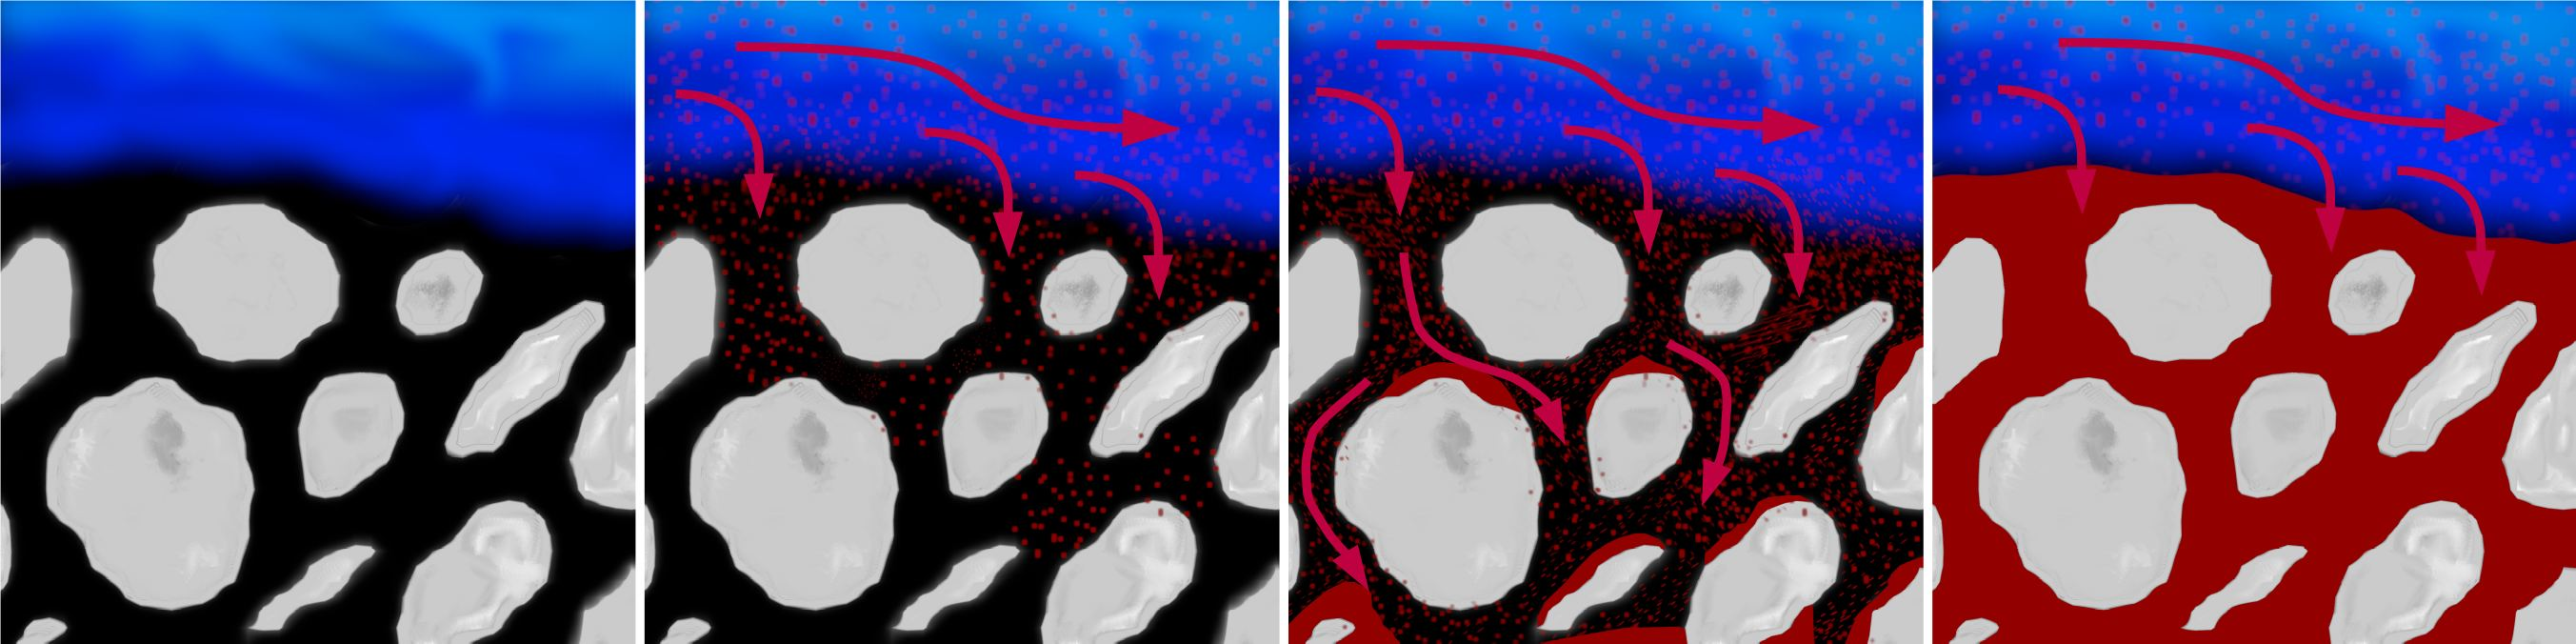
\includegraphics[width=0.91\paperwidth]{new-clogging-assembley-1}};
		\end{scope}}
		\onslide<2->{
		\node[anchor=south west, xshift=0.33\paperwidth, yshift=0.225\paperheight, text=black, text width=0.5\paperwidth,align=left]{\tiny Image concept adapted from \sscURL{Schälchli (1993)}{https://ethz.ch/content/dam/ethz/special-interest/baug/vaw/vaw-dam/documents/das-institut/mitteilungen/1990-1999/124.pdf}};}
	\end{tikzpicture}
\end{frame}


\subsection{Riverbed Clogging Measurement Methods}

\begin{frame}{\secname\vspace{0.1cm}\\\textcolor{anthrazit!80!white}{\subsecname}}\vspace{-0.8cm}
	\begin{columns}[T]
		\begin{column}{.5\textwidth}
			\sscFig{multipac}{The Multi-Parameter Approach for
				assessing riverbed Clogging (MultiPAC -- \sscURL{Negreiros \textit{et al.}, 2023}{https://onlinelibrary.wiley.com/doi/abs/10.1002/rra.4145}; \sscURL{Seitz, 2020}{http://dx.doi.org/10.18419/opus-11249}. Imagery: \sscURL{Schwindt \textit{et al.}, 2023}{https://www.sciencedirect.com/science/article/pii/S1470160X23011871})}
		\end{column}\hspace{-0.5cm}
		\begin{column}{.4313\textwidth}\vspace{0.77cm}
			\onslide<1->{
				\sscFig{sfm-freeze-core-19}{MultiPAC measurements at the Inn}\vspace{-0.5cm}
			}
			\onslide<2->{
				\faHandORight\ \textbf{Grain sizes, porosity, interstitial dissolved oxygen concentration (IDOC), hydraulic conductivity}}
		\end{column}
	\end{columns}
	% \textbf{Water temperature, filter velocity (for hydraulic conductivity), pH value,\\\hspace{0.4cm} interstitial dissolved oxygen}}
\end{frame}

\subsection{Engineering Solutions to Reinstate Vertical Connectivity Locally}
\begin{frame}{\secname\vspace{0.1cm}\\\textcolor{anthrazit!80!white}{\subsecname}}
	\begin{tikzpicture}
		\clip (0,0) rectangle (\paperwidth,\paperheight);
		\onslide<1->{
		\begin{scope}
				\node[anchor=south west, xshift=0.0\paperwidth, yshift=0.295\paperheight] {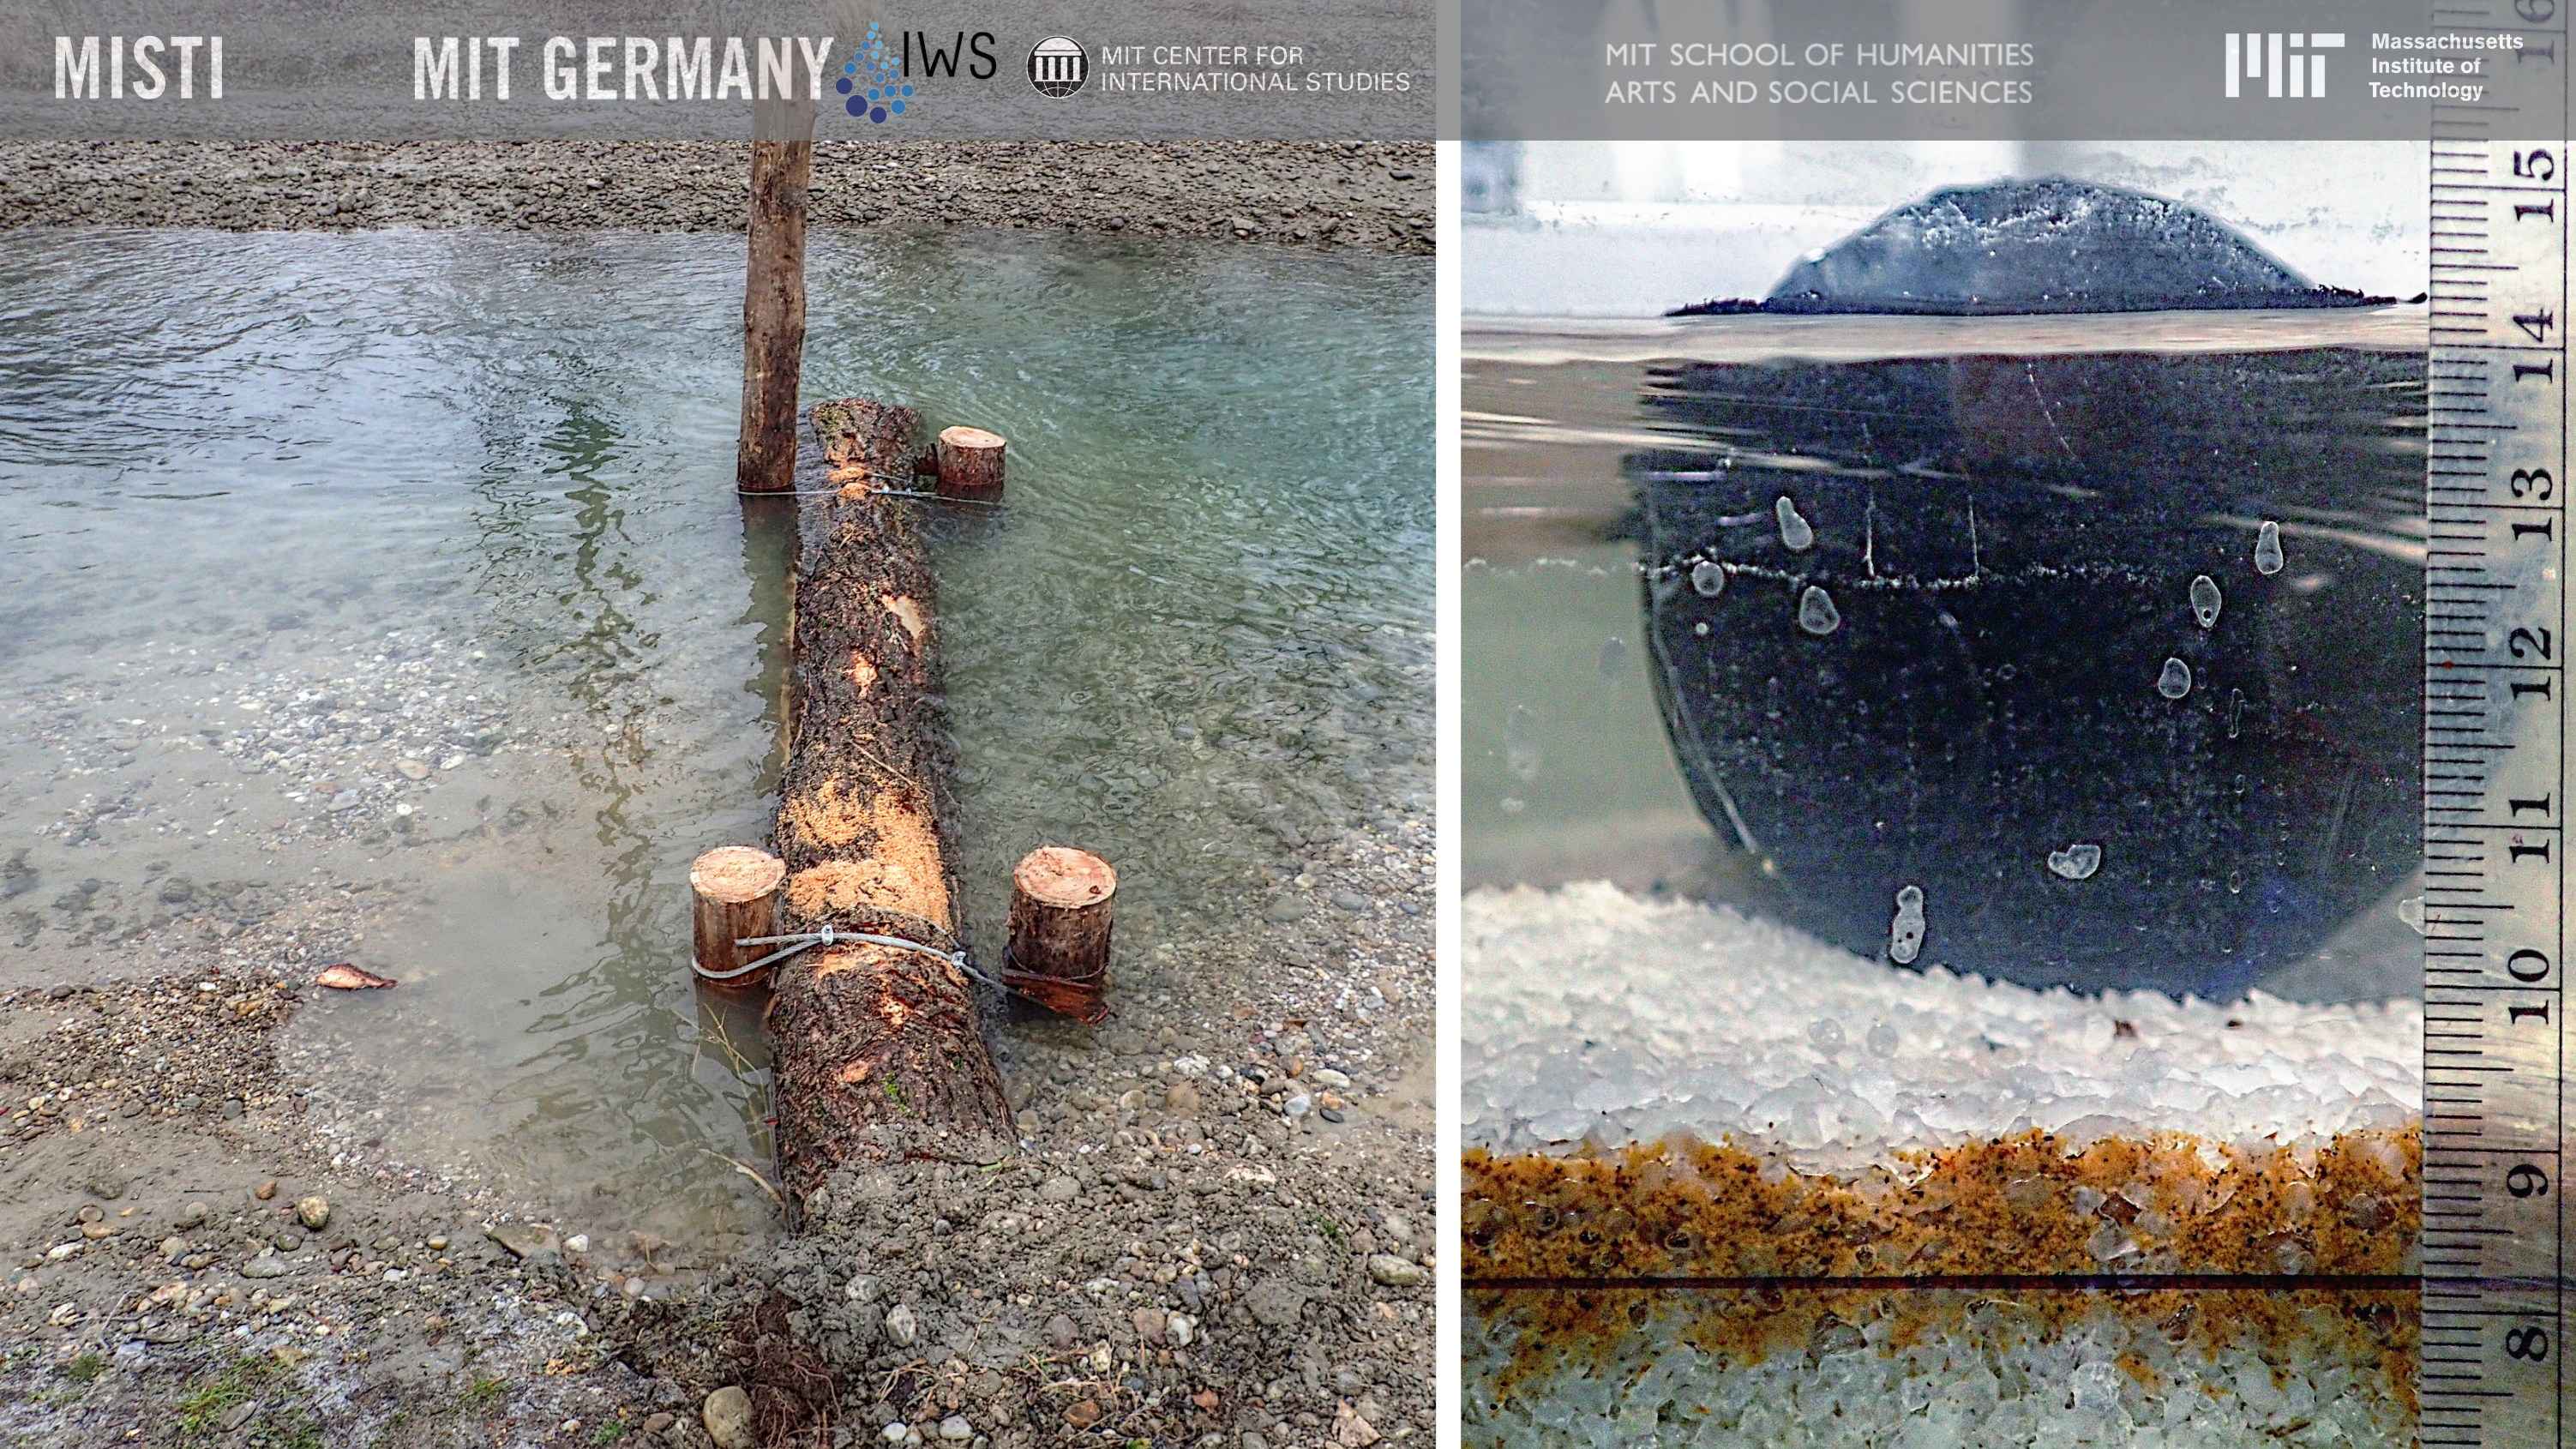
\includegraphics[width=0.86\paperwidth]{lwm-experiment}};
		\end{scope}}
	%	\onslide<1->{
	%		\node[anchor=south west, xshift=0.33\paperwidth, yshift=0.225\paperheight, text=black, text width=0.5\paperwidth,align=left]{\tiny Images adapted from Schwindt \textit{et al.} (2023, subm.)};}
	\end{tikzpicture}
\end{frame}


\begin{frame}{\secname\vspace{0.1cm}\\\textcolor{anthrazit!80!white}{\subsecname}}
	\begin{tikzpicture}
		\clip (0,0) rectangle (\paperwidth,\paperheight);
		\onslide<1->{
		\begin{scope}
				\node[anchor=south west, xshift=0.0\paperwidth, yshift=0.25\paperheight] {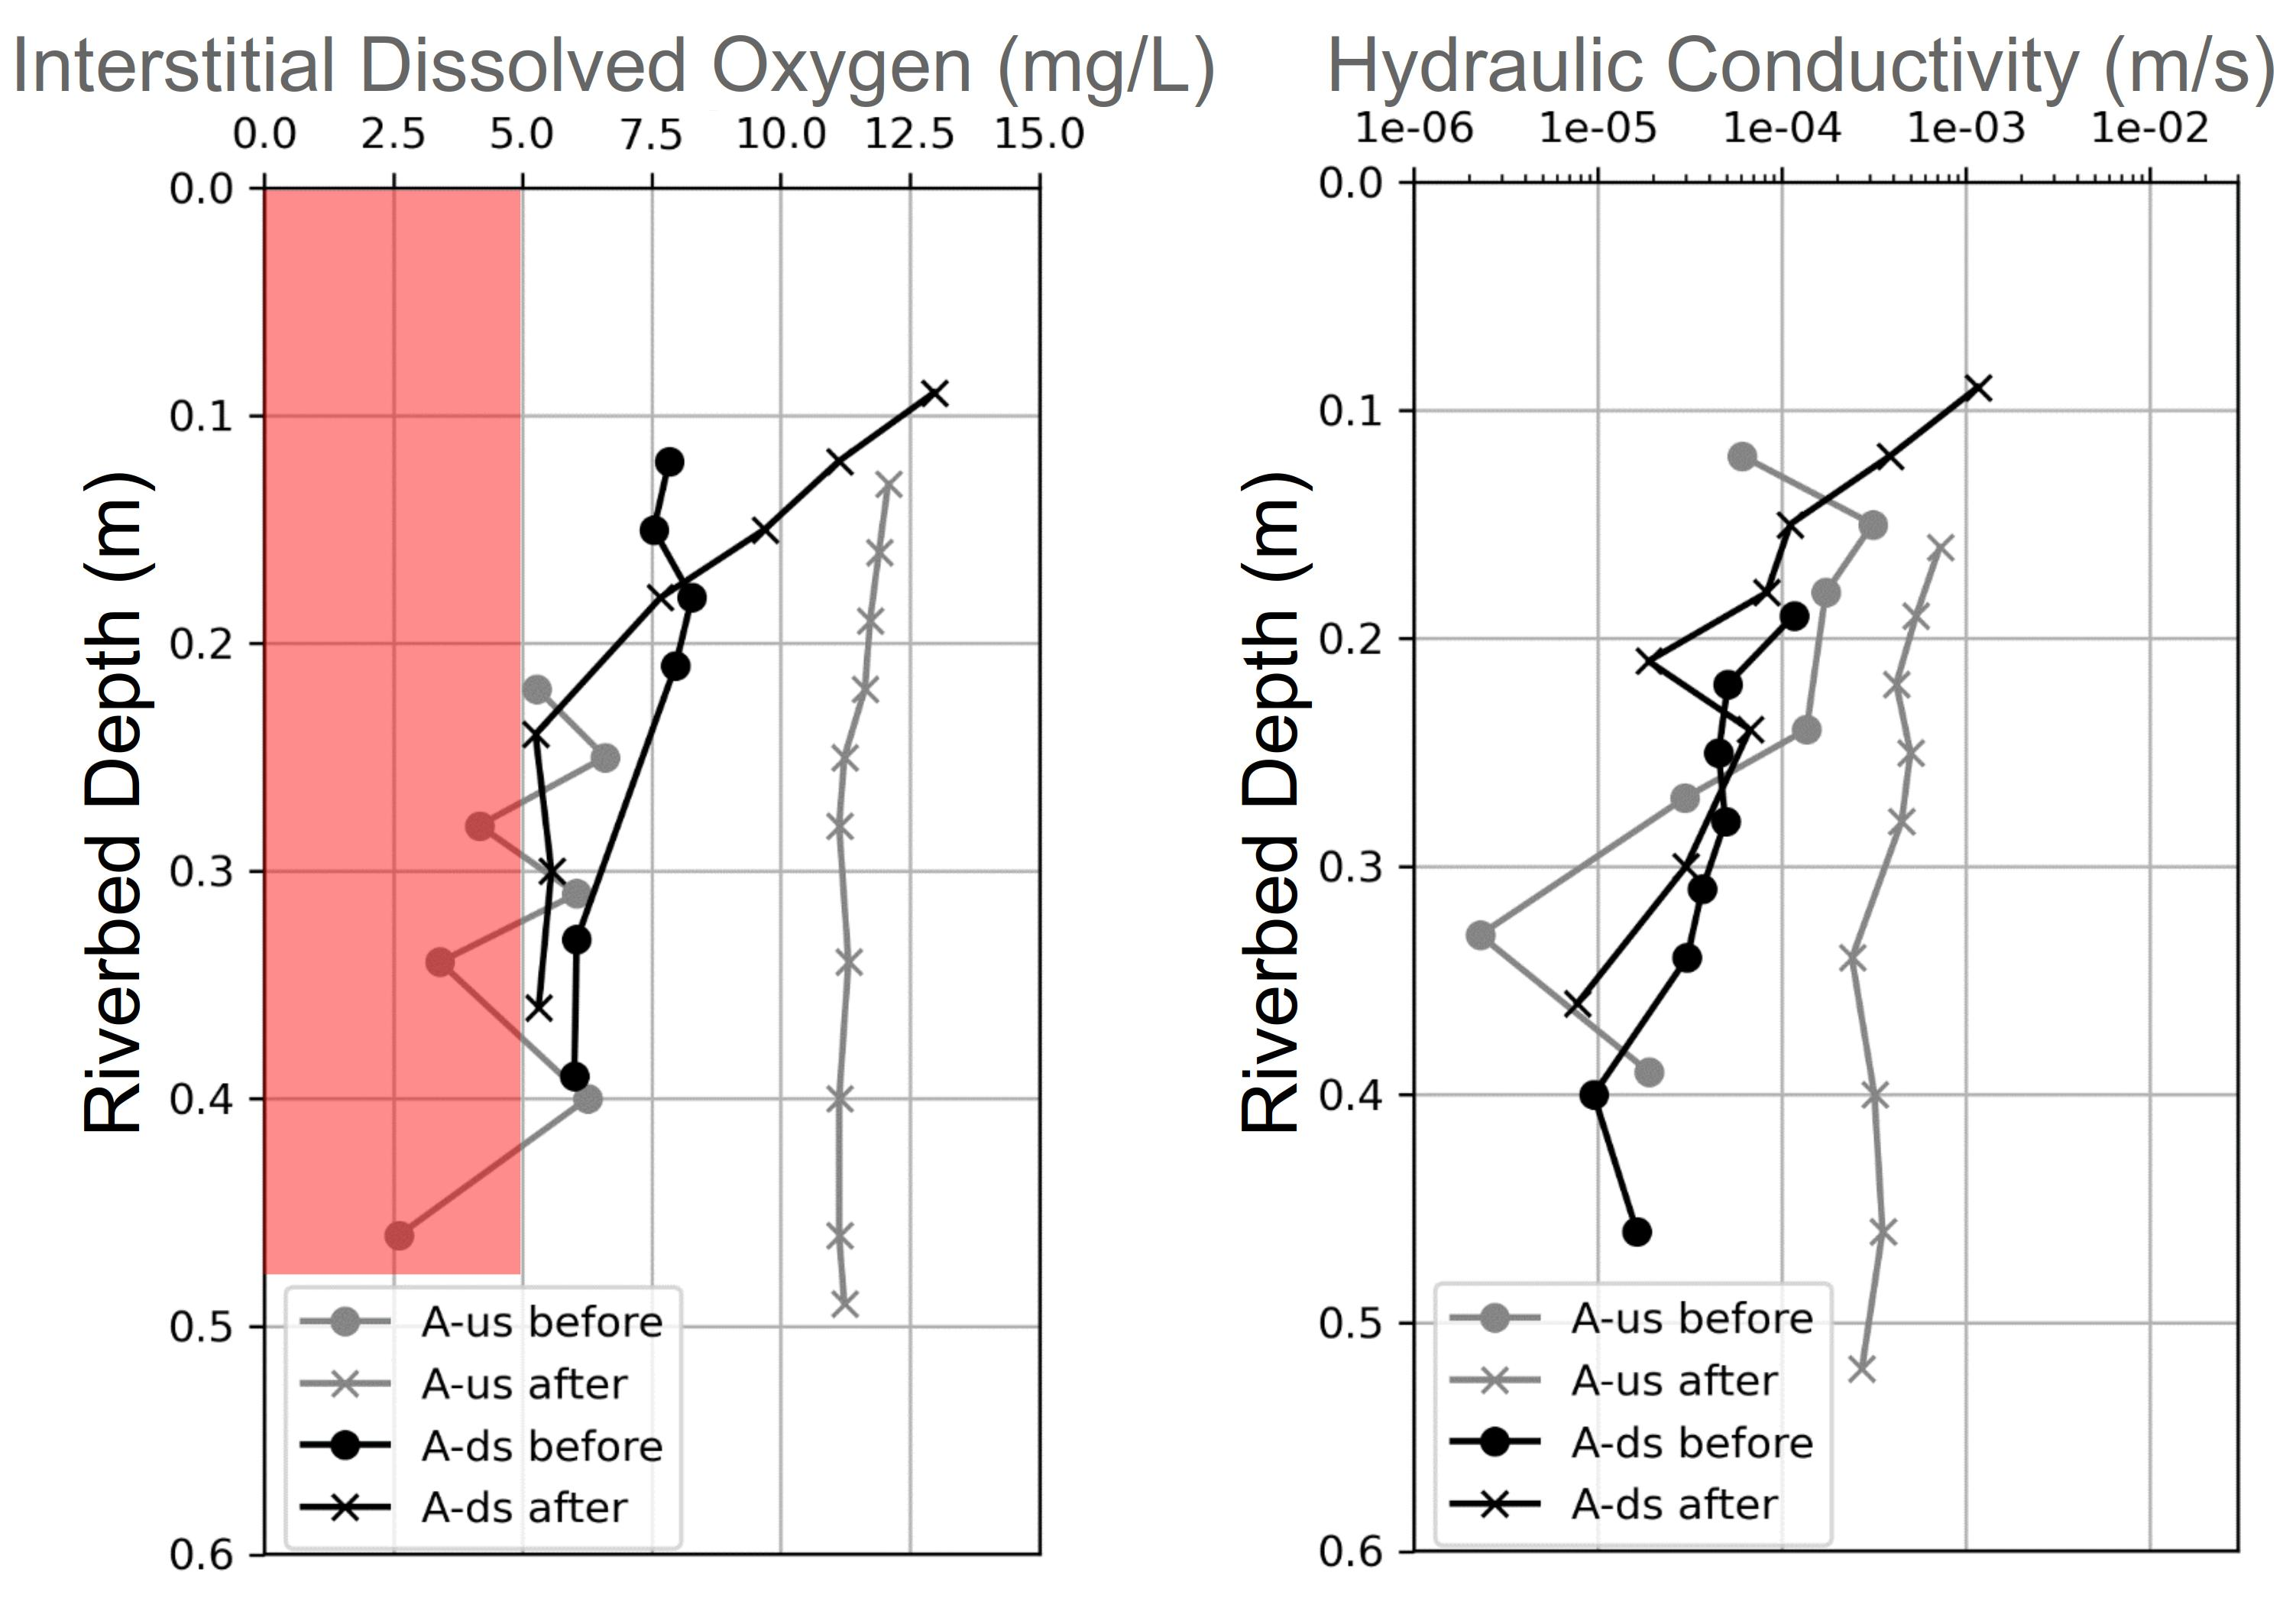
\includegraphics[width=0.8\paperwidth]{idoc-kf-results}};
		\end{scope}
		}
		\onslide<1->{
			\node[anchor=south west, xshift=0.33\paperwidth, yshift=0.225\paperheight, text=black, text width=0.5\paperwidth,align=left]{\tiny Images adapted from \sscURL{Schwindt \textit{et al.}, 2023}{https://www.sciencedirect.com/science/article/pii/S1470160X23011871}};
			}
	\end{tikzpicture}
\end{frame}

{
\usebackgroundtemplate{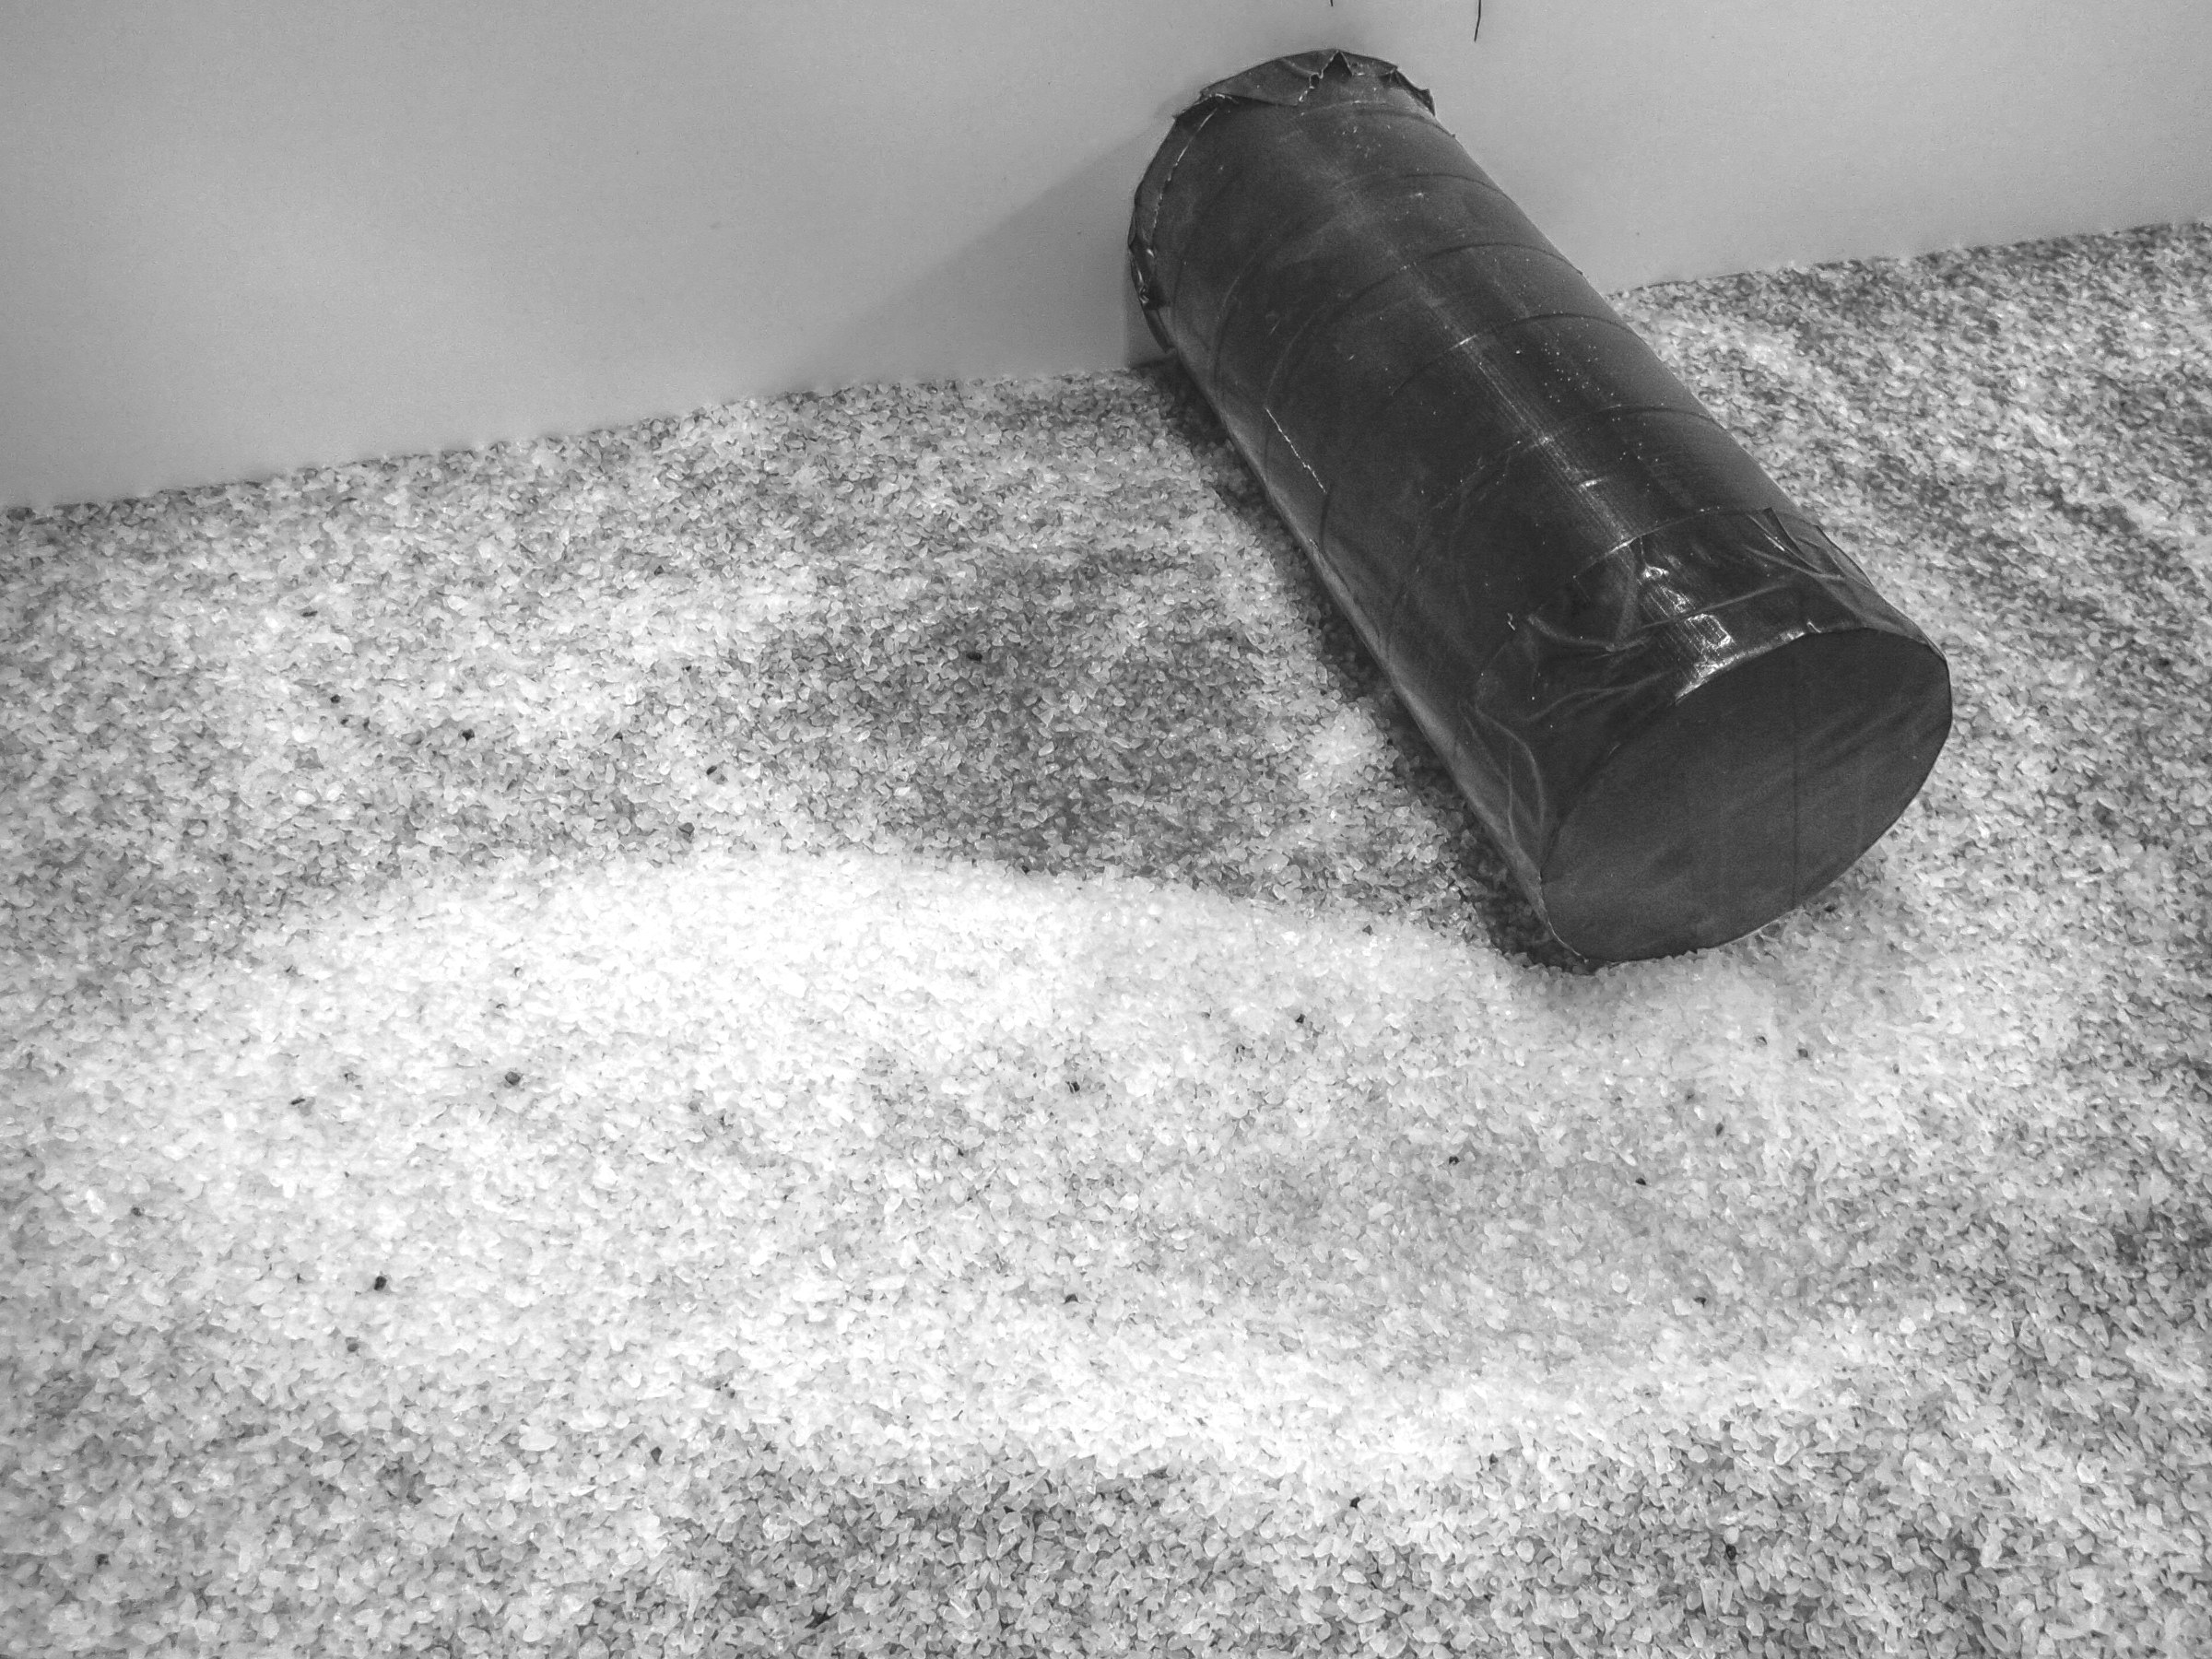
\includegraphics[width=\paperwidth]{test2-observations-18}}%
\begin{frame}[plain]{}{\secname}
	\vspace{3cm}
	\onslide<1->{
		\begin{tcolorbox}[colbacktitle=hellblau!80!black, colback=hellblau!10!white, fonttitle=\bfseries, standard jigsaw,colframe=blue_light, bottom=0mm, middle=0mm, boxsep=0.2mm, opacityframe=0.5, opacityfill=0.85, opacitybacktitle=0.95, title filled, title={Insights from the Nepf Lab}, size=fbox]
			\vspace{0.25cm}
			\begin{itemize}
				\item[\faChevronCircleRight]\ Emergent logs have higher declogging effect
				\item[\faChevronCircleRight]\ Elevated declogging in the wake of the tip of the logs
			\end{itemize}
			\vspace{0.25cm}
			{\small
				\begin{flushright}
				  \sscURL{Schalko/Ponce, Lassar, Schwindt, Haun, Nepf 2024}{https://www.nature.com/articles/s41598-023-47501-1}
				\end{flushright}
			}
		\end{tcolorbox}\smallskip}
\end{frame}}

%\begin{frame}{\secname\vspace{0.1cm}\\\textcolor{anthrazit!80!white}{\subsecname}}
%	\begin{tikzpicture}
%		\clip (0,0) rectangle (\paperwidth,\paperheight);
%			\begin{scope}
%				\begin{tcolorbox}[colbacktitle=hellblau!80!black, colback=hellblau!15!white, fonttitle=\bfseries, standard jigsaw,colframe=blue_light, bottom=0mm, middle=0mm, boxsep=0.2mm, opacityframe=0.5, opacityfill=0.75, opacitybacktitle=0.95, title filled, title={Insights from the Nepf Lab}, size=fbox]
%					\vspace{0.25cm}	 
%					\begin{itemize}
%						\item[\faChevronCircleRight]\ Emergent logs have higher declogging effect
%						\item[\faChevronCircleRight]\ Elevated declogging in the wake of submerged logs
%					\end{itemize}
%					\vspace{0.25cm}
%					{\tiny Images adapted from \sscURL{Schalko/Ponce \textit{et al.}, 2024}{https://www.nature.com/articles/s41598-023-47501-1}}
%				\end{tcolorbox}\smallskip
%			\end{scope}
%
%	\end{tikzpicture}
%\end{frame}


\subsection{Combined Vertical and Lateral Connectivity}
\begin{frame}{\secname\vspace{0.1cm}\\\textcolor{anthrazit!80!white}{\subsecname}}
	Reconnecting the y-axis: bank removal
	\begin{tikzpicture}
		\clip (0,0) rectangle (\paperwidth,\paperheight);
		\onslide<1->{
			\begin{scope}
				\node[anchor=south west, xshift=0.\paperwidth, yshift=0.295\paperheight] {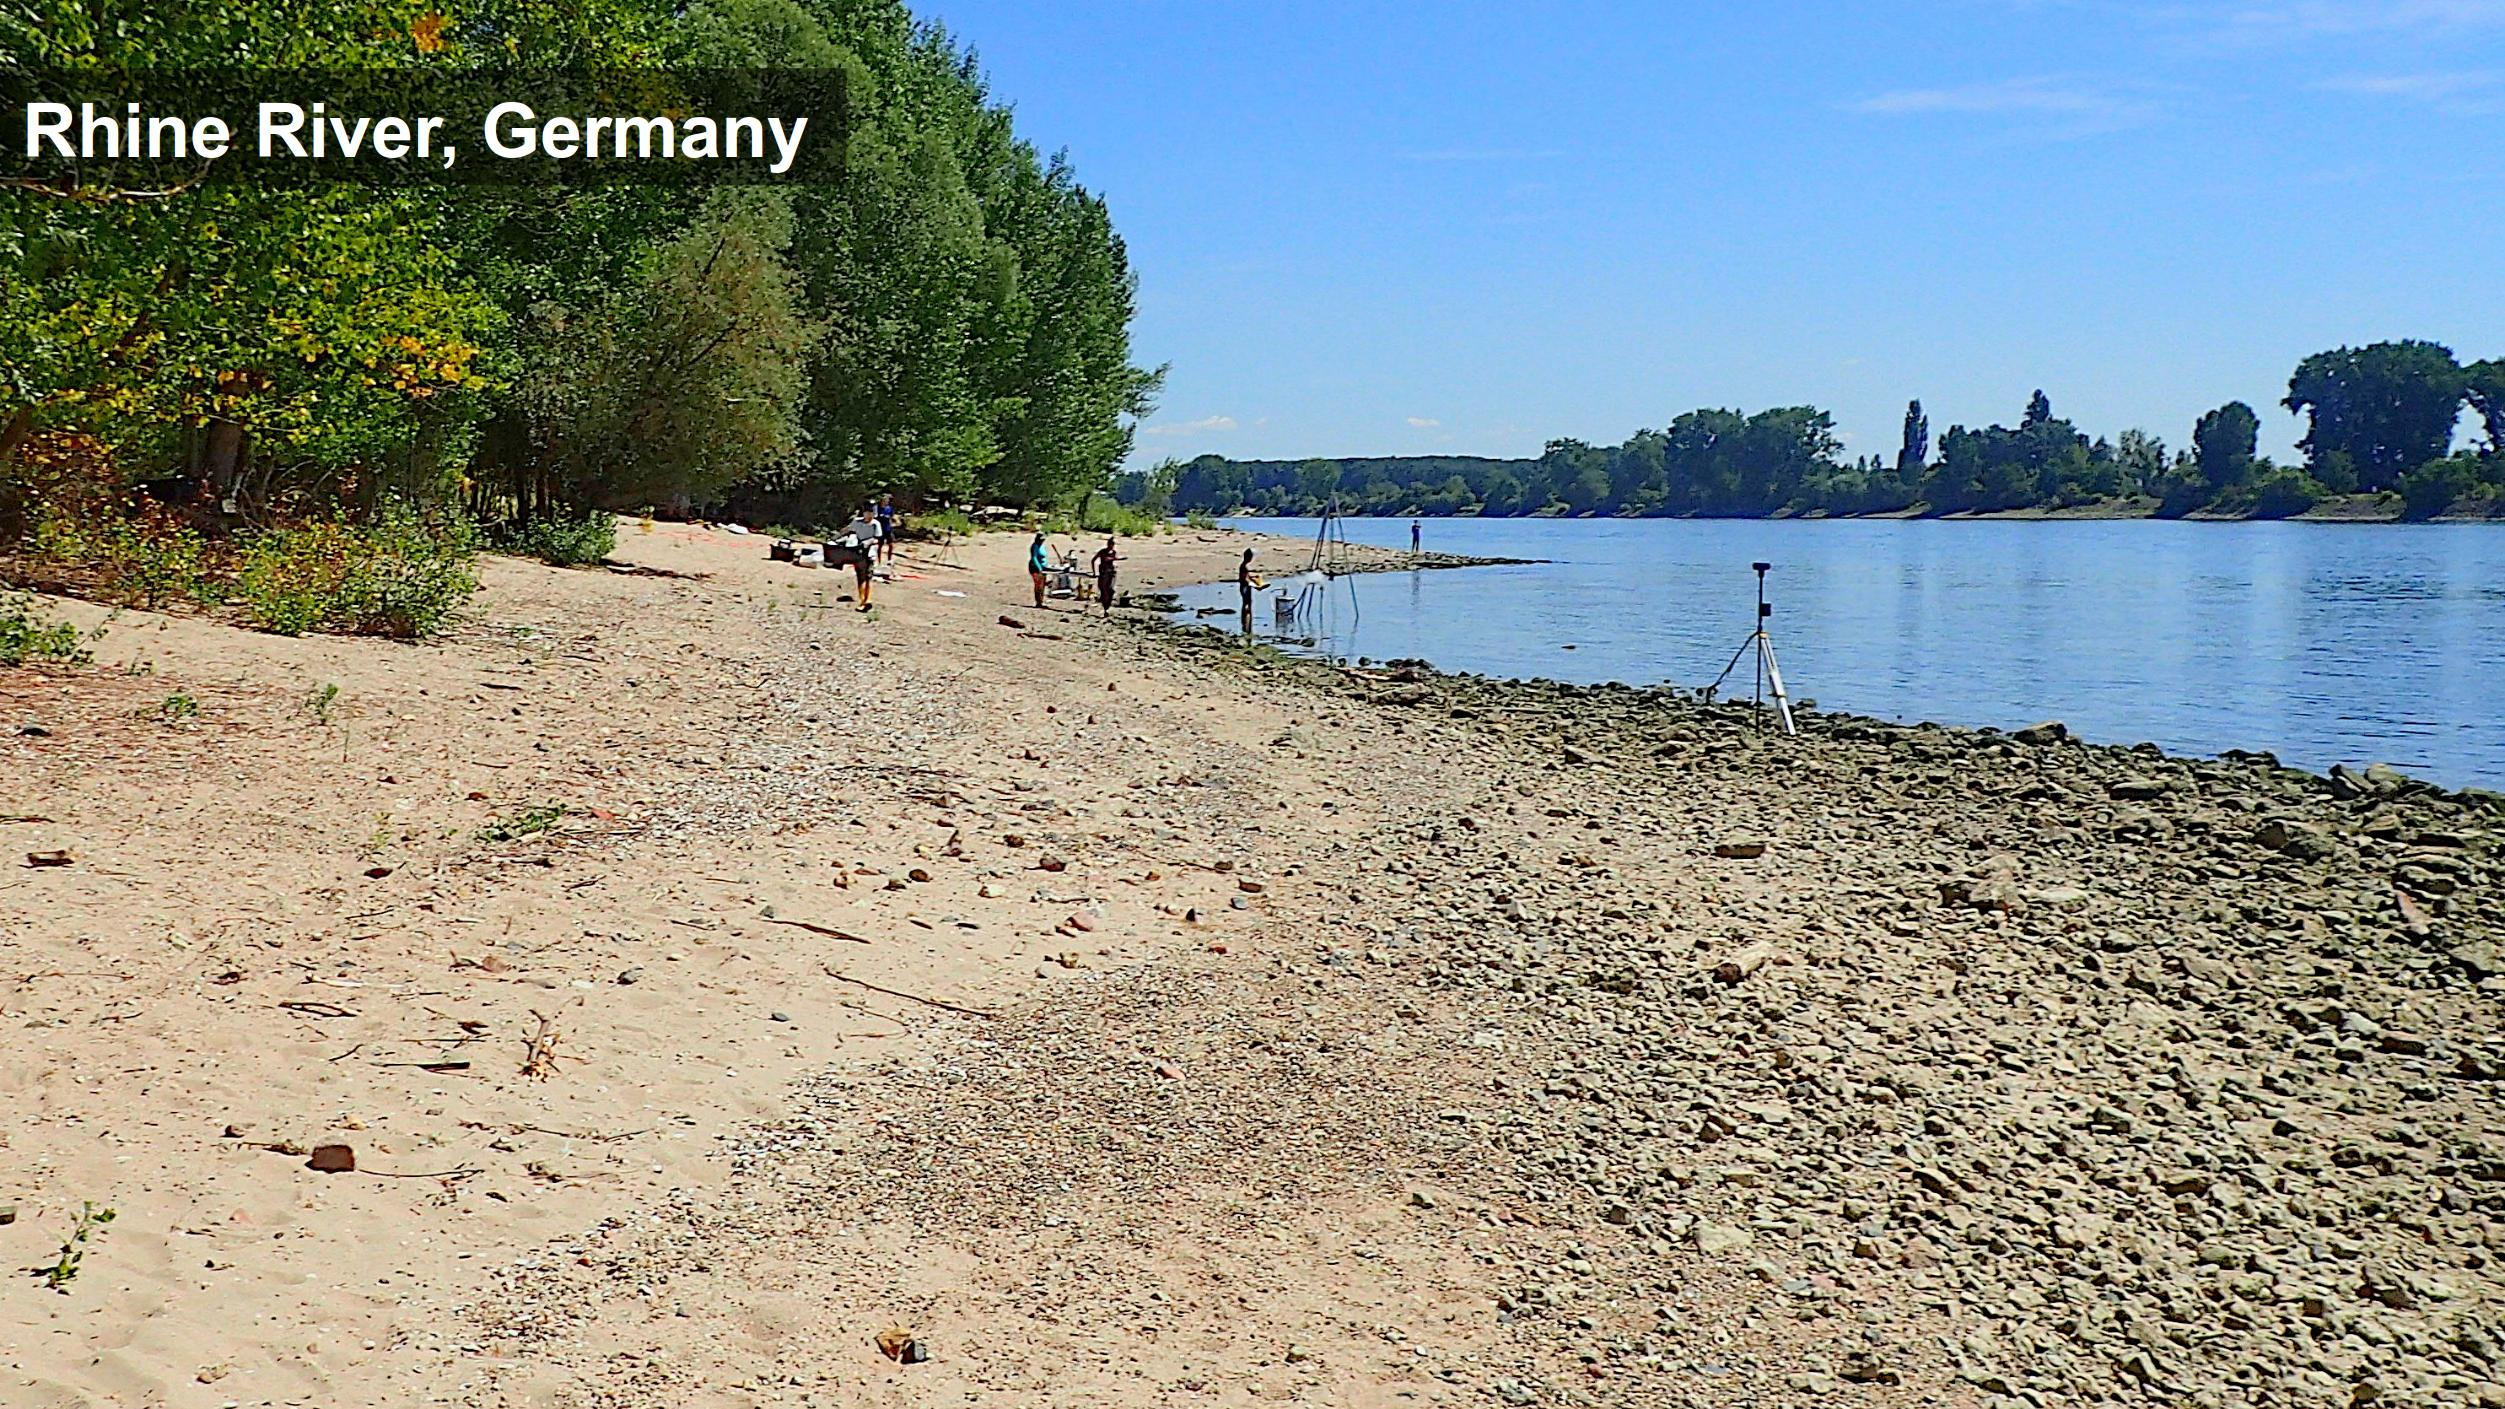
\includegraphics[width=0.86\paperwidth]{rhine-bank-removal-0}};
		\end{scope}}
		\onslide<2->{
			\begin{scope}
				\node[anchor=south west, xshift=0.\paperwidth, yshift=0.295\paperheight] {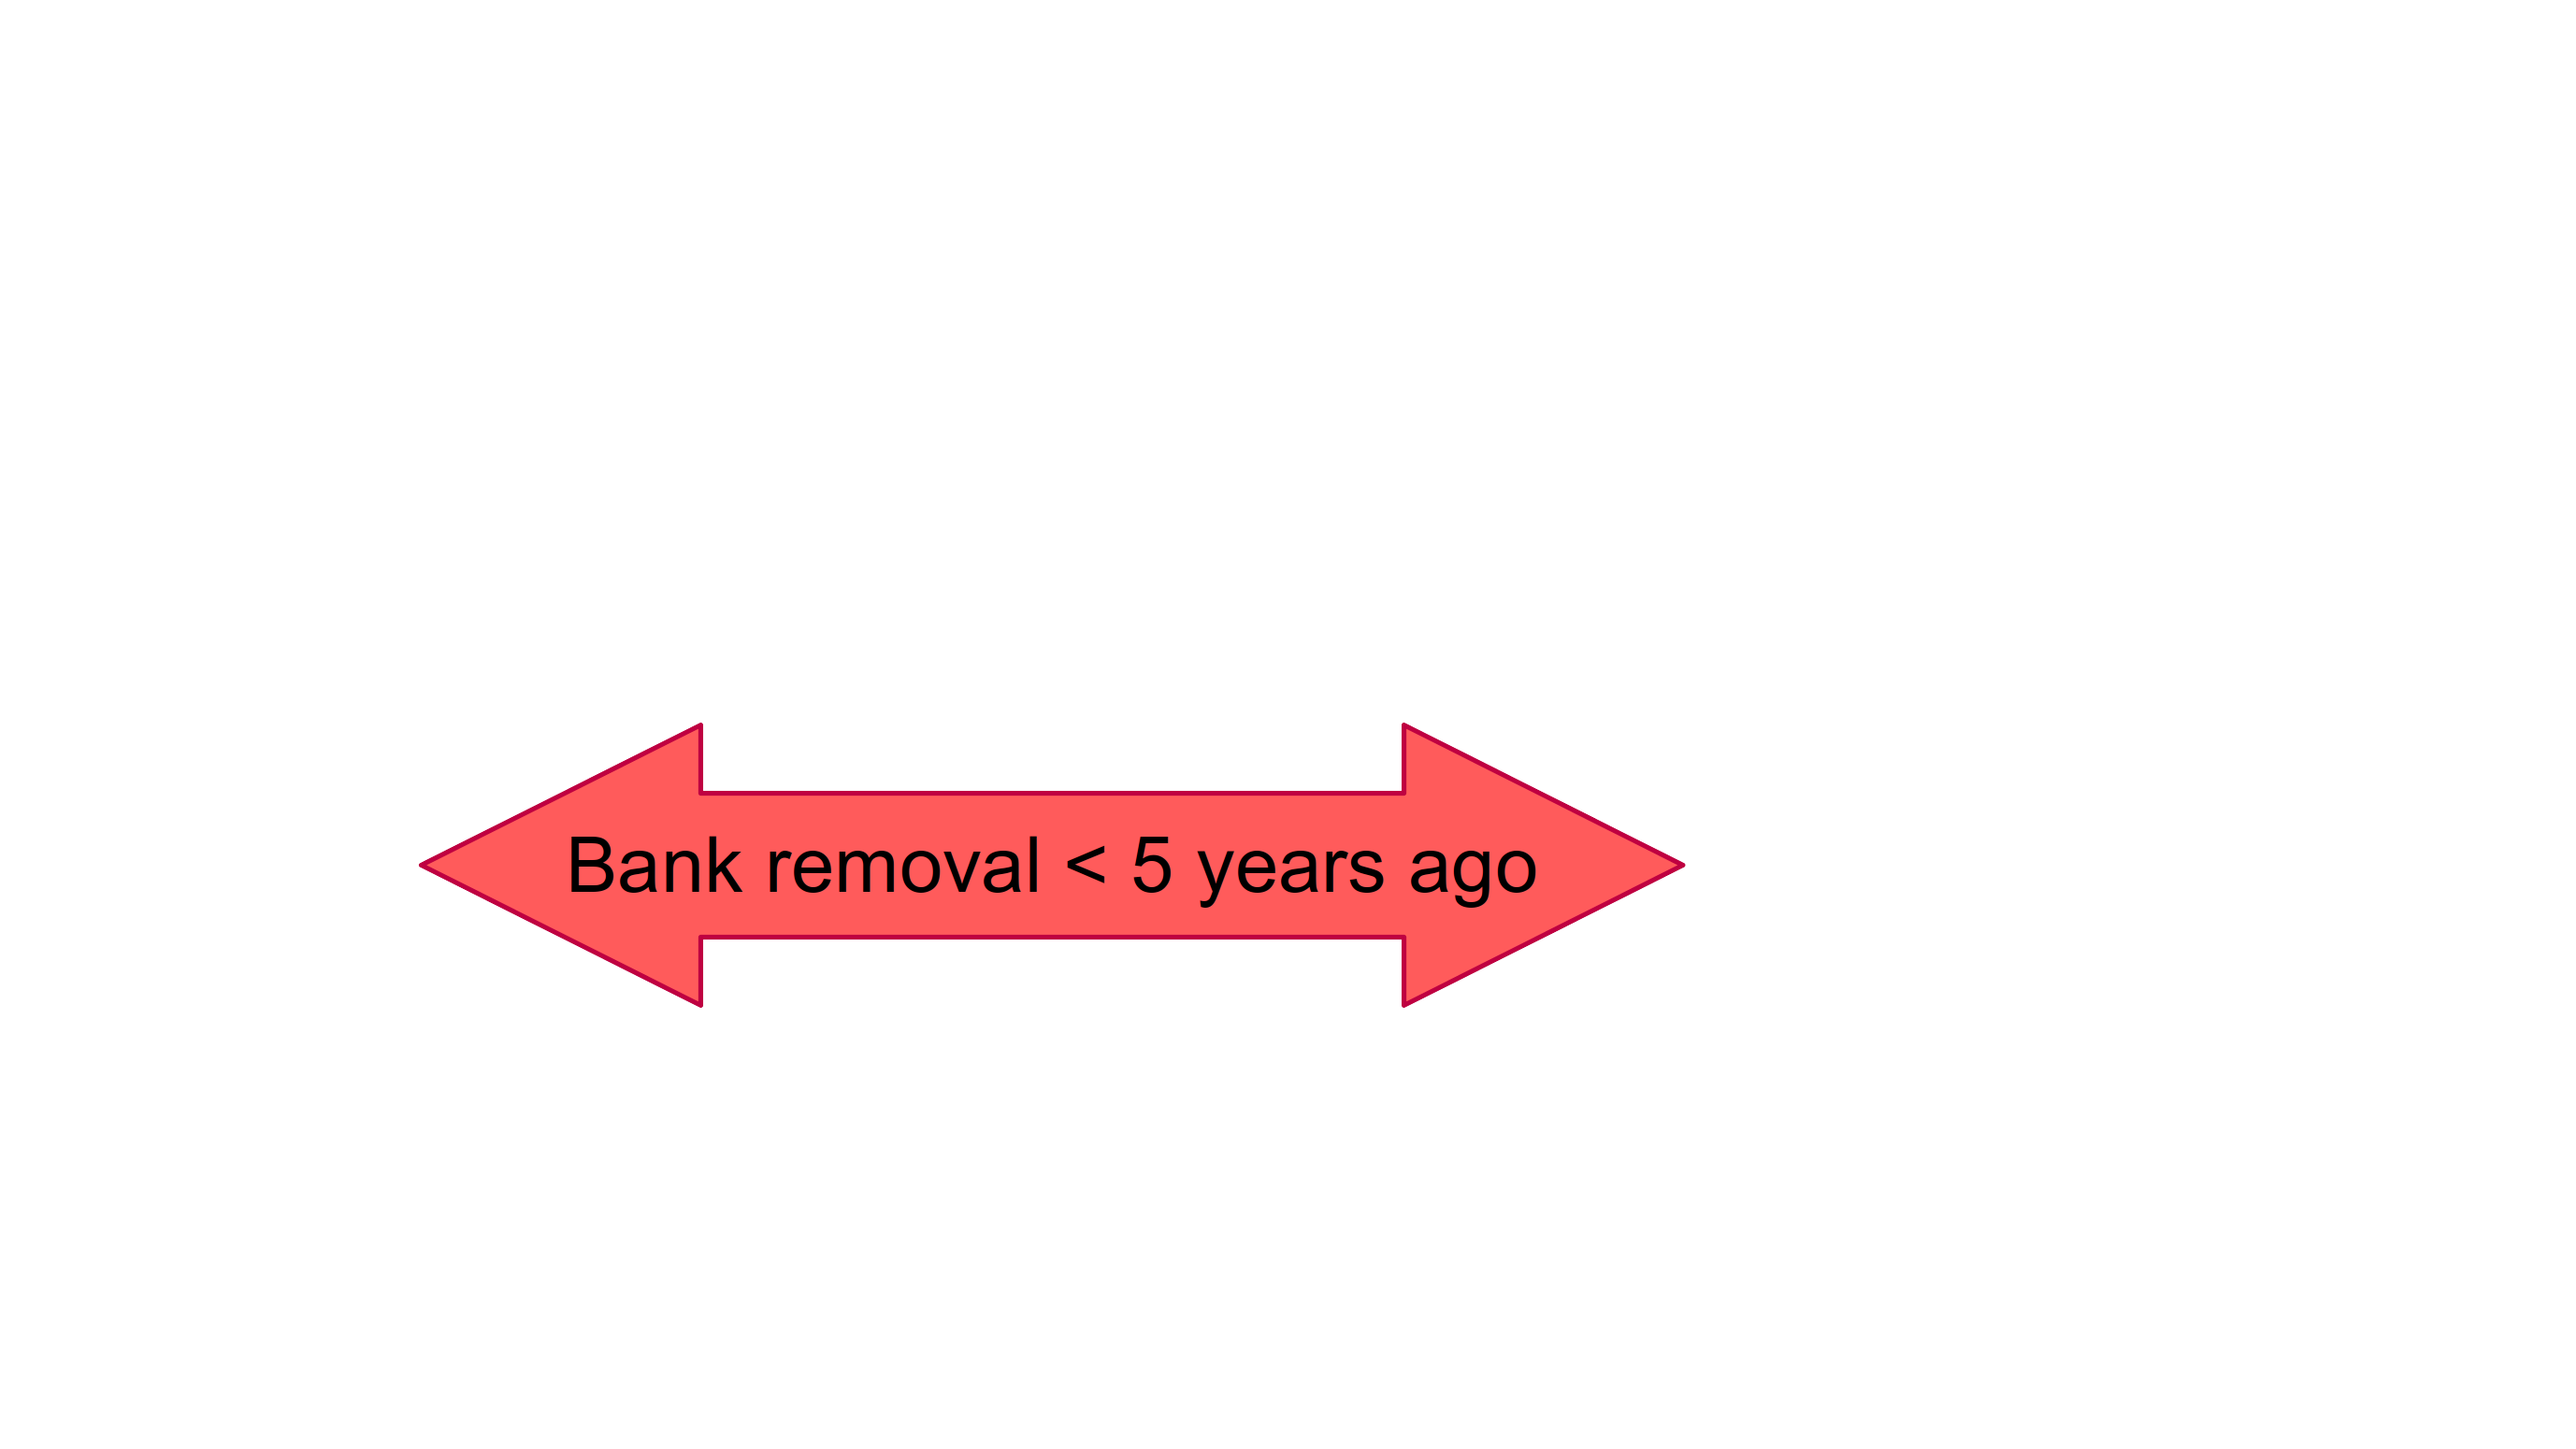
\includegraphics[width=0.86\paperwidth]{rhine-bank-removal-1}};
		\end{scope}}
	\end{tikzpicture}
\end{frame}

\begin{frame}{\secname\vspace{0.1cm}\\\textcolor{anthrazit!80!white}{\subsecname}}
	\begin{tikzpicture}
		\clip (0,0) rectangle (\paperwidth,\paperheight);
		\onslide<1->{
		\begin{scope}
			\node[anchor=south west, xshift=0.0\paperwidth, yshift=0.27\paperheight] {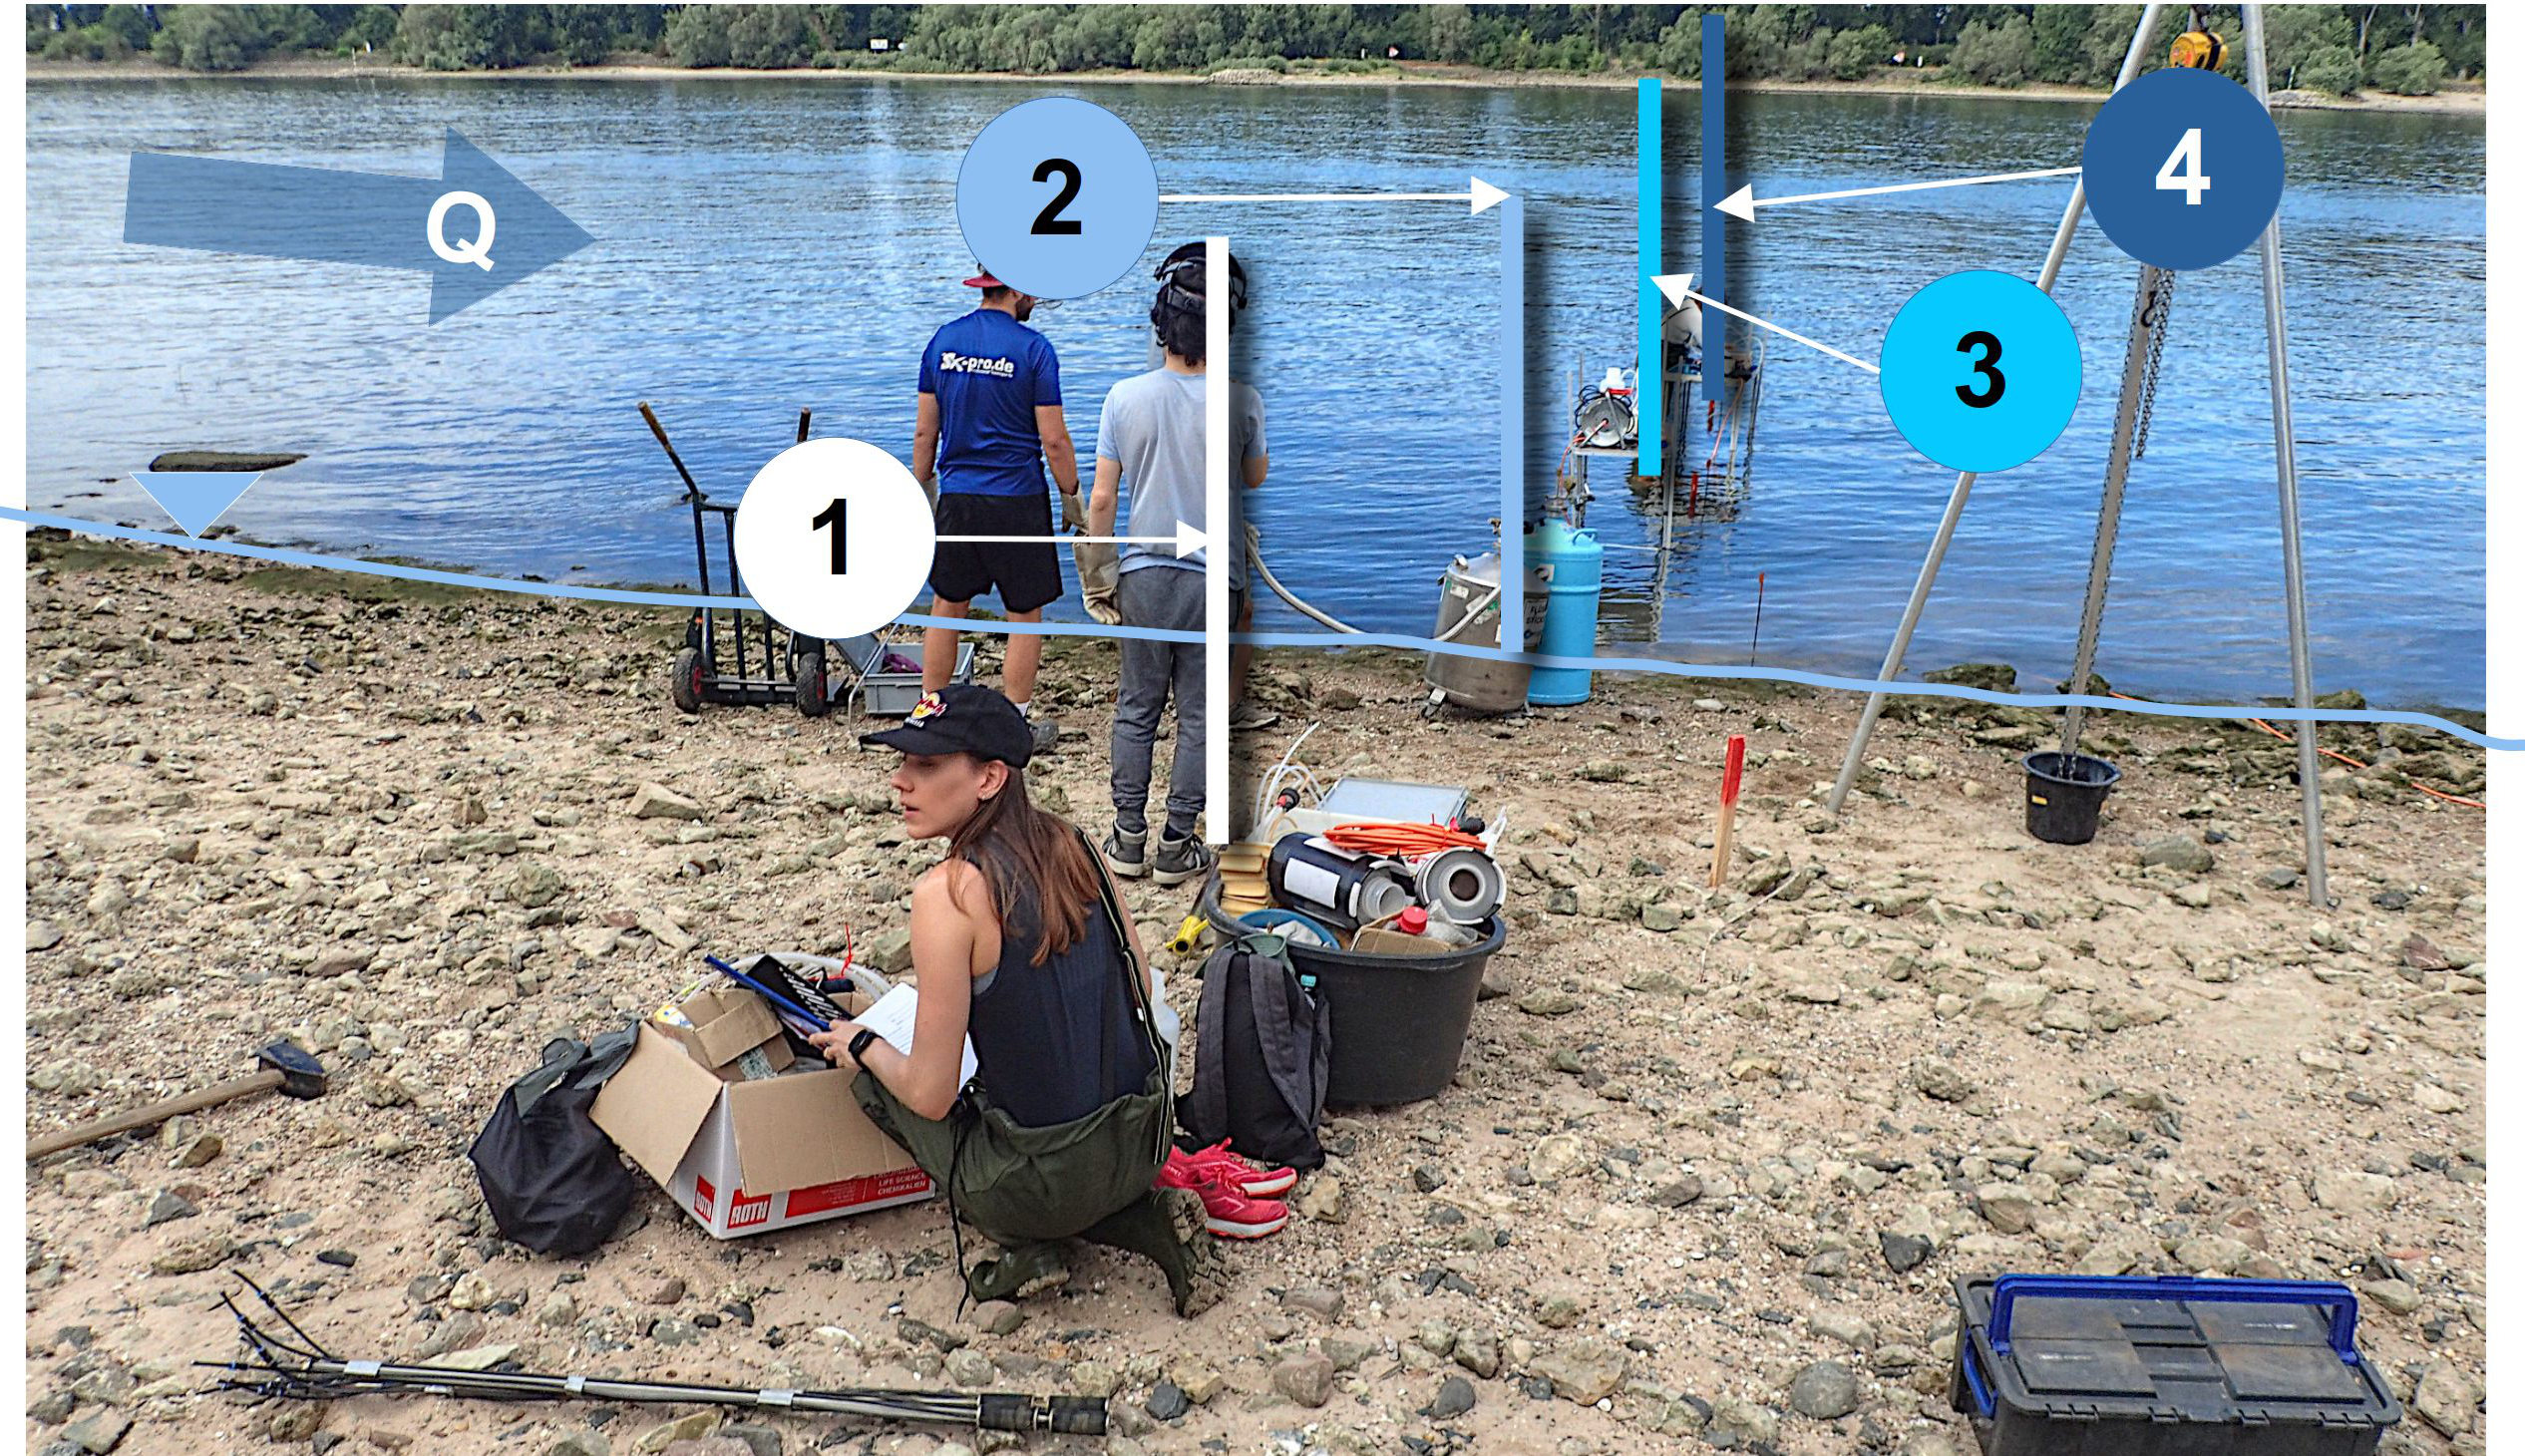
\includegraphics[width=0.88\paperwidth]{multipac-rhine}};
		\end{scope}}
	\end{tikzpicture}
\end{frame}



\begin{frame}{\secname\vspace{0.1cm}\\\textcolor{anthrazit!80!white}{\subsecname}}
	\begin{tikzpicture}
		\clip (0,0) rectangle (\paperwidth,\paperheight);
		\onslide<1->{
			\begin{scope}
				\node[anchor=south west, xshift=0.0\paperwidth, yshift=0.31\paperheight] {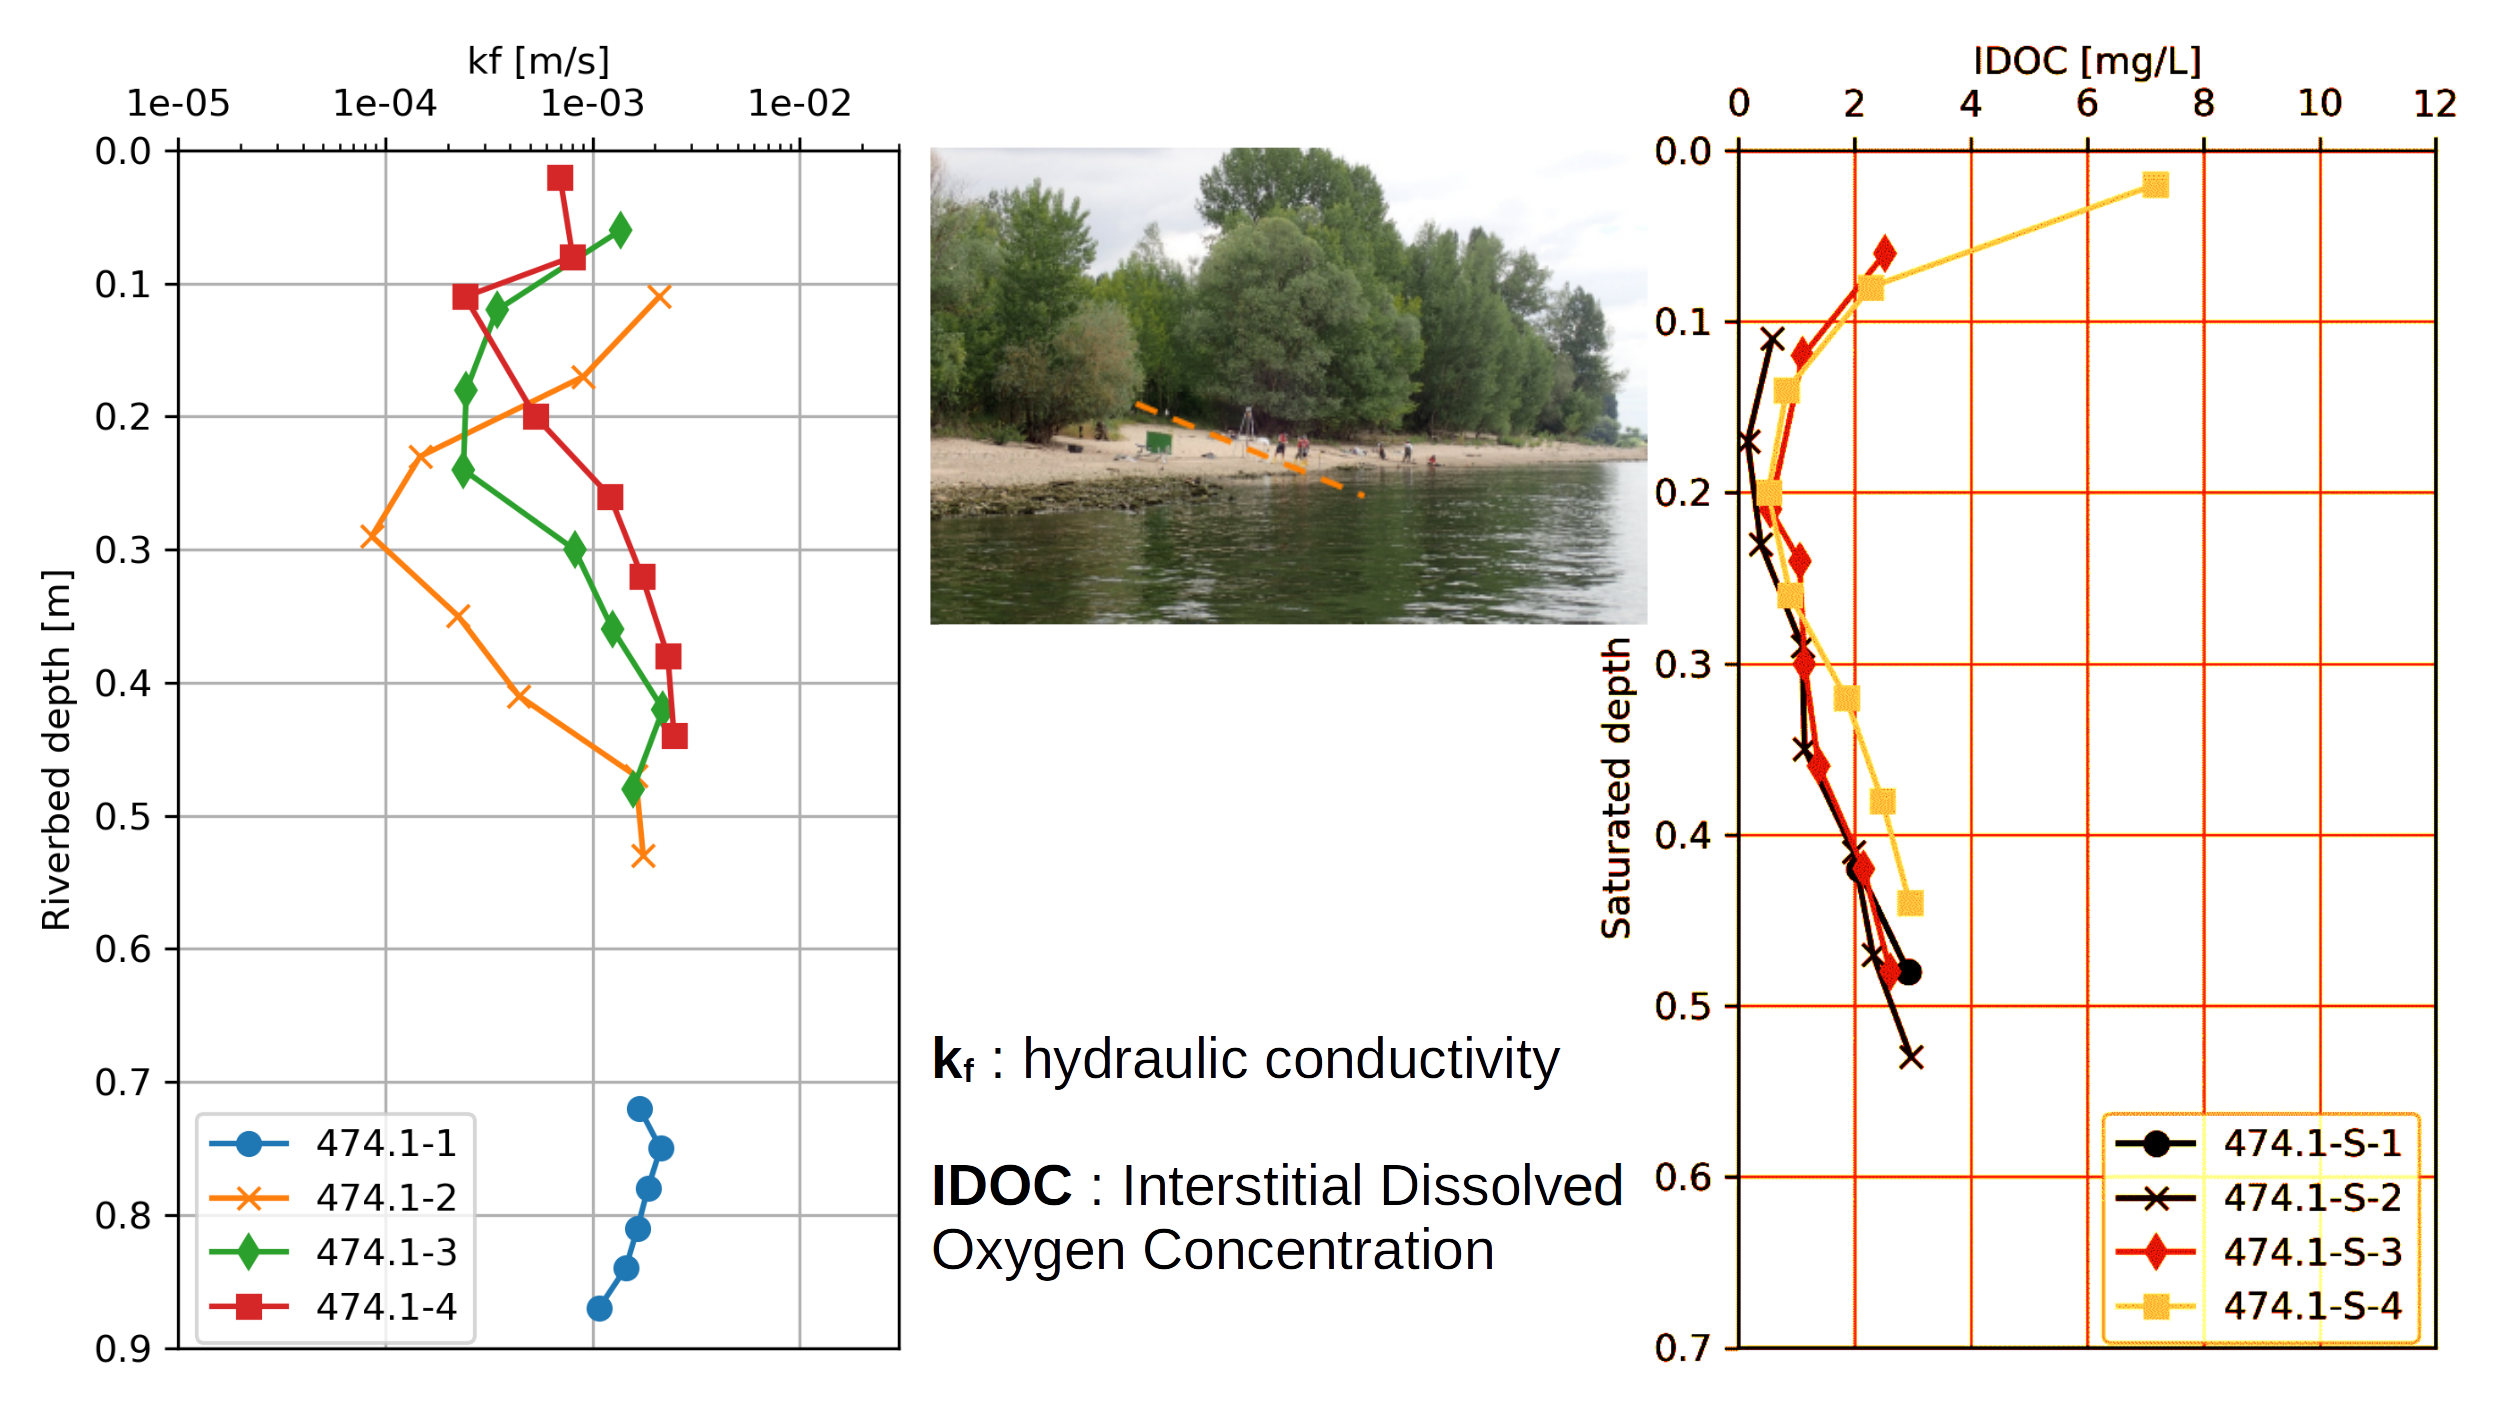
\includegraphics[width=0.9\paperwidth]{rhine-profiles-full}};
		\end{scope}}
	\end{tikzpicture}
\end{frame}


\begin{frame}{\secname\vspace{0.1cm}\\\textcolor{anthrazit!80!white}{\subsecname}}
	\begin{tikzpicture}
		\clip (0,0) rectangle (\paperwidth,\paperheight);
		\onslide<1->{
			\begin{scope}
				\node[anchor=south west, xshift=0.0\paperwidth, yshift=0.31\paperheight] {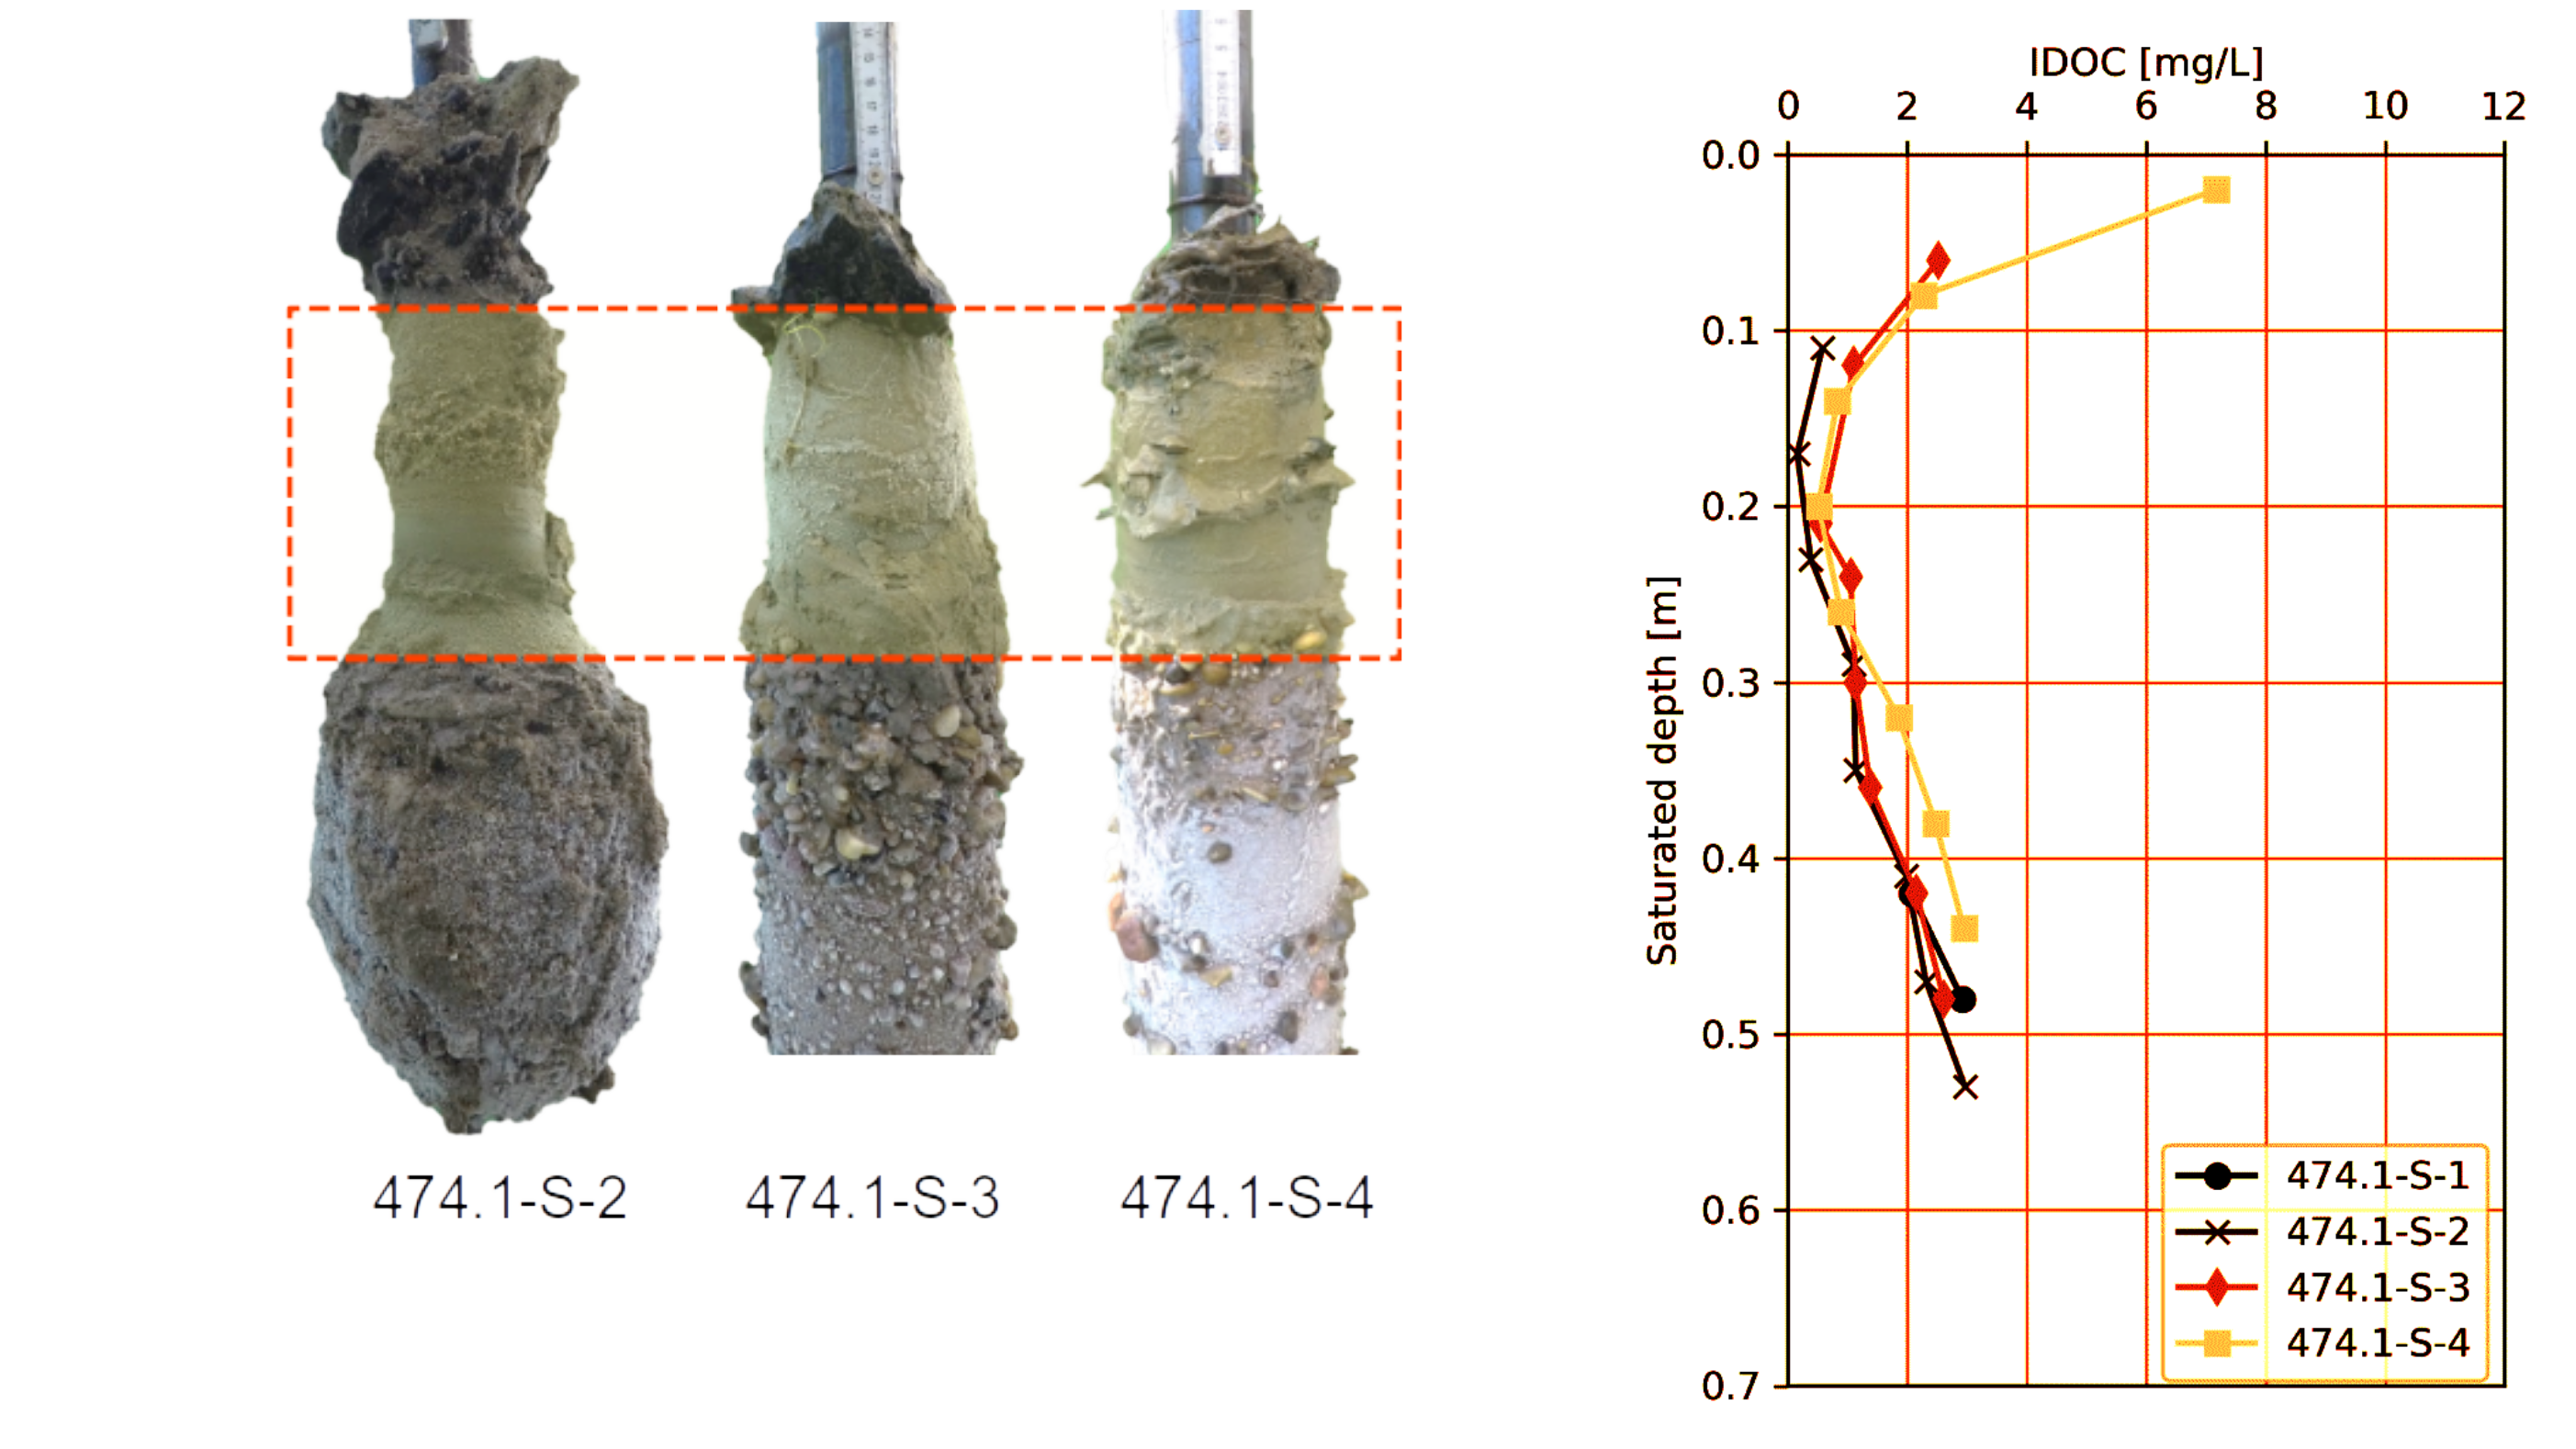
\includegraphics[width=0.9\paperwidth]{rhine-profiles-analysis}};
		\end{scope}}
	\end{tikzpicture}
\end{frame}


\begin{frame}{\secname\vspace{0.1cm}\\\textcolor{anthrazit!80!white}{\subsecname}}
	\begin{tikzpicture}
		\clip (0,0) rectangle (\paperwidth,\paperheight);
		\onslide<1->{
		\begin{scope}
				\node[anchor=south west, xshift=0.0\paperwidth, yshift=0.31\paperheight] {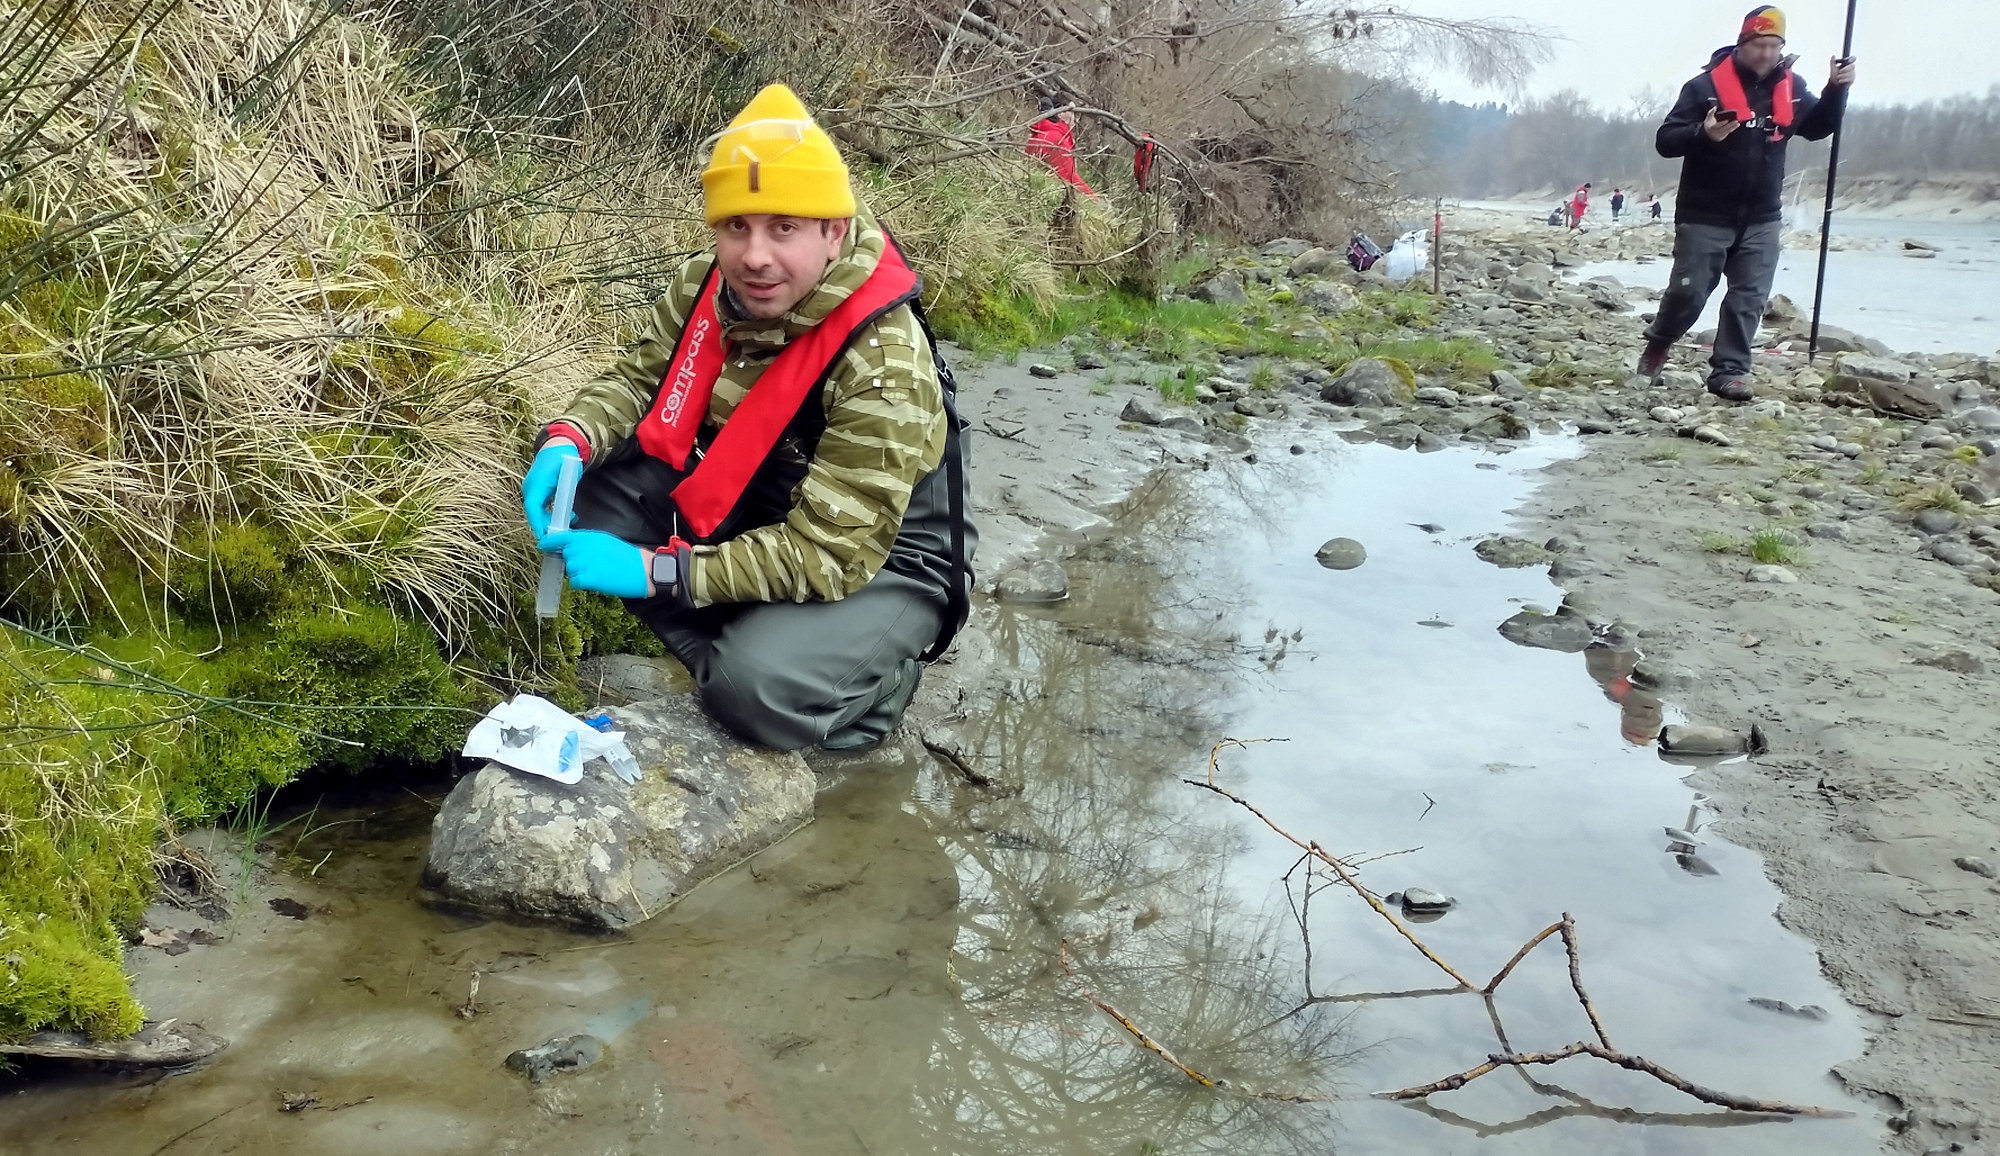
\includegraphics[width=0.88\paperwidth]{inn-new-campaign}};
		\end{scope}
		\begin{scope}
			\node[anchor=south west, xshift=0.0\paperwidth, yshift=0.31\paperheight] {
\includegraphics[width=0.88\paperwidth]{inn-new-campaign-overlay}};
		\end{scope}}
	\end{tikzpicture}
\end{frame}
